В даной главе анализируются свойства предложенных моделей и рекомендации по их использованию. Качество полученных моделей сравнивается с качеством
известных решений.
\section{Выбор модели классификации временных рядов}

В данном разделе рассматривается задача построения сети глубокого обучения для классификации временных рядов. Под временным рядом понимается реализация некоторого случайного процессса.  Работы~\cite{ts1,ts2,ts3} посвящены классификации временных рядов с использованием методов глубокого обучения. В работе~\cite{ts2}  для классификации временных рядов  используются рекуррентные нейронные сети. В работе~\cite{ts3} рассматриваются различные суперпозиции ограниченной машины Больцмана, автокодировщика и двуслойной нейронной сети. Исследуется суперпозиция, состоящая из ограниченной машины Больцмана, автокодировщика и двуслойной нейронной сети~\cite{founds}. Работа~\cite{recrbm} посвящена рекуррентной модификации модели ограниченной машины Больцмана для классификации временных рядов. 

В данном разделе решается прикладная задача классификации временных рядов. В качестве данных для вычислительного эксперимента используются данные с акселерометров мобильных телефонов~\cite{wisdm}. Для решения задачи оптимизации используется алгоритм обратного распространения ошибок с послойным предобучением сети и дальнейшей настройкой параметров всех слоев~\cite{finetuning}.

\textbf{Постановка задачи. }
Рассматривается задача классификации. 
Моделью классификации  $\mathbf{f}$ выступает суперпозиция подмоделей, аналогичная~\eqref{eq:softmax_example}:
\begin{equation}
\label{eq:wisdm_superposition}
 \mathbf{f}(\mathbf{w}, \mathbf{x}) = \mathbf{f}_1(\mathbf{f}_2(\dots \mathbf{f}_{|V|}(\mathbf{x}))): \mathbb{R}^n \to [0,1]^R,
\end{equation}
где $\mathbf{f}_v, v \in \{1,\dots,{|V|}\}$ --- модели, параметрическое семейство вектор-функции; $\mathbf{w}$ --- вектор параметров моделей;
$c$-ю компоненту вектора $\mathbf{f}(\mathbf{x},\mathbf{w})$ будем интерпретировать как вероятность отнесения объекта $\mathbf{x}_i$ к классу с меткой $c$~\eqref{eq:proba_softmax}.

Требуется минимизировать функцию ошибки $L$ на обучающей выборке $\mathfrak{D}$,
где $L$ --- сумма отрицательных логарифмов правдоподобия по всем объектам выборки
\[
\mathbf{w}^{*} = \argmin_\mathbf{w} L(\mathbf{w}|\mathfrak{D}),
\]
где
\[
 L(\mathbf{w}|\mathfrak{D}) = -\sum_{i=1}^m \sum_{r=1}^R [y_i = r] \text{log} p(y_i=r|\mathbf{x}_i,\mathbf{w}).
\]

\textbf{Структура сети глубокого обучения. }
Предлагается использовать в качестве алгоритма решения задачи суперпозицию, состоящую из трех основных компонент:
ограниченной машины Больцмана, автокодировщика и двуслойной нейросети с softmax-классификатором.
Модель~\eqref{eq:wisdm_superposition} в данном случае выглядит следующим образом:
\[
    \mathbf{f}(\mathbf{w}, \mathbf{x}) = \mathbf{f}_\text{SM} \cdot \mathbf{f}_\text{AE} \cdot  \mathbf{f}_\text{RBM}(\mathbf{x}),
\]
где $\mathbf{f}_\text{RBM}, \mathbf{f}_\text{AE}, \mathbf{f}_\text{SM}$ --- модели ограниченной машины Больцмана, автокодировщика и двуслойной нейронной сети соответственно.

\textbf{Ограниченная машина Больцмана.}
Ограниченная машина Больцмана представляет собой двудольный граф, где первая доля соответствует переменной $\mathbf{x}$, а вторая доля --- бинарному вектору $\mathbf{h}$ длины $n'$.
% \begin{equation}\end{equation}
Рассмотрим случай, когда вектор $\mathbf{x}$ принимает бинарные значения. Определим энергию пары входного слоя $\mathbf{x}$ и скрытого слоя $\mathbf{h}$ следующим образом:
\[
 E(\mathbf{x},\mathbf{h}) = -\mathbf{x}^\text{T} \cdot \mathbf{b}_\text{vis} -\mathbf{h}^\mathsf{T} \cdot \mathbf{b}_\text{hid} - \mathbf{h}^\mathsf{T}\mathbf{w}_\text{RBM}\mathbf{x},
\]
где $\mathbf{b}_\text{vis}, \mathbf{b}_\text{hid}, \mathbf{w}_\text{RBM}$ --- параметры модели.

Пусть совместное распределение пары векторов $\mathbf{x}, \mathbf{h}$ задано следующим образом:
\[
	p(\mathbf{x}, \mathbf{h}) = \frac{1}{Z} \text{exp}\bigl(-E(\mathbf{x},\mathbf{h})\bigr),
\]
где $Z$ --- нормировочный коэффициент:
\[
 Z = \sum_{\mathbf{x} \in \{0,1\}^n} \sum_{\mathbf{h}\in \{0,1\}^{n'}} \text{exp}\bigl(-E(\mathbf{x},\mathbf{h})\bigr).
\]


Функция вероятностей вектора $\mathbf{x}$ есть сумма вероятностей по всем скрытым состояниям вектора $\mathbf{h}$:
\[
	p(\mathbf{x}) = \sum_{\mathbf{h}\in \{0,1\}^{n'}} p(\mathbf{x}, \mathbf{h}).
\]

Определим элемент суперпозиции~\eqref{eq:wisdm_superposition}: 
\begin{equation}
\label{eq:rbm_model}
\mathbf{f}_\text{RBM}(\mathbf{x}) = \mathsf{E}(\mathbf{h}|\mathbf{x}).
\end{equation}
Параметры модели~\eqref{eq:rbm_model} оптимизируются следующим образом:
\begin{equation}
\label{eq:rbm}
{\mathbf{w}}^{*}_\text{RBM},{\mathbf{b}}^{*}_\text{vis}, {\mathbf{b}}^{*}_\text{hid} = \argmax_{{\mathbf{w}_\text{RBM}},{\mathbf{b}}_\text{vis}, {\mathbf{b}}_\text{hid} } p(\mathbf{X}, [{\mathbf{w}_\text{RBM}},{\mathbf{b}}_\text{vis}, {\mathbf{b}}_\text{hid}]) = \prod_{i=1}^m \sum_{\mathbf{h}\in \{0,1\}^{n'}} \frac{1}{J} \text{exp}\bigl(-E(\mathbf{\mathbf{x}_i},\mathbf{h)}\bigr).
\end{equation}
В данной работе используется модифицированная версия ограниченной машины Больцмана, позволяющая работать с небинарными входными данными~\cite{gbrbm}. В этой модификации энергия $E$ пары входного слоя $\mathbf{x}$ и скрытого слоя $\mathbf{h}$ выглядит следующим образом:
\[
E(\mathbf{x},\mathbf{h}) = \frac{(\mathbf{x} - \mathbf{b}_\text{vis})^2}{2\hat{\boldsymbol{\sigma}}]^2} -\mathbf{h}^\mathsf{T} \cdot \mathbf{b}_\text{hid} - \frac{\mathbf{h}}{\hat{\boldsymbol{\sigma}}}^\mathsf{T}\mathbf{w}_\text{RBM}\mathbf{x},
\]
где $\hat{\boldsymbol{\sigma}}$ --- эмпирическая оценка среднеквдратичного отклонения по выборке $\mathbf{X}$, деление производится покомпонентно. 


Для решения задачи оптимизации~\eqref{eq:rbm} используется алгоритм, описанный в~\cite{hinton_rbm}.

\textbf{Автокодировщик.}
Автокодировщик предназначен для снижения размерности исходного пространства признаков.
Автокодировщик представляет собой суперпозицию кодирующего и декодирующего блока:
\[
 \mathbf{f}_\text{AE}' = \mathbf{f}_\text{enc}(\mathbf{f}_\text{dec}(\mathbf{x})),
\]
где $$ \mathbf{f}_\text{enc}(\mathbf{x}) = \boldsymbol{\sigma}(\mathbf{w}_\text{enc}\mathbf{x}+\mathbf{b}_\text{enc}) \text{ --- кодирующий блок,}$$
$$  \mathbf{f}_\text{dec}(\mathbf{x}) = \boldsymbol{\sigma}(\mathbf{w}_\text{dec}\mathbf{g}(\mathbf{x})+\mathbf{b}_\text{dec})\text{ --- декодирующий блок,}$$ $$\boldsymbol{\sigma}(x) = (1+\textbf{exp}({-\mathbf{x}}))^{-1} \text{ --- сигмоидная функция},$$ $\mathbf{w}_\text{enc},\mathbf{w}_\text{dec},\mathbf{b}_\text{enc}, \mathbf{b}_\text{dec}$ --- параметры модели.

Введем дополнительное ограничение на матрицы $\mathbf{w}_\text{enc}, \mathbf{w}_\text{dec}$:
\[
 \mathbf{w}_\text{enc} = \mathbf{w}_\text{dec}^{^\mathsf{T}}.
\]

Параметры $\mathbf{w}_\text{enc}, \mathbf{w}_\text{dec}, \mathbf{b}_\text{enc}, \mathbf{b}_\text{dec}$ оптимизируются так, чтобы по образу вектора $\mathbf{x}$ получить восстановленный вектор $\mathbf{f}_\text{AE}'$, близкий к исходному $\mathbf{x}$:
\begin{equation}
\label{eq:ae}
 \mathbf{w}^{*}_\text{enc},\mathbf{w}^{*}_\text{dec},\mathbf{b}^{*}_\text{enc}, \mathbf{b}^{*}_\text{dec} = \argmin_{{\mathbf{w}}_\text{enc},{\mathbf{w}}_\text{dec},{\mathbf{b}}_\text{enc}, {\mathbf{b}}_\text{dec}} \frac{1}{m}\sum_{i=1}^m ||\mathbf{f}_\text{AE}'(\mathbf{x}_i)-\mathbf{x}_i||^2_2.
\end{equation}

Декодирующий блок $\mathbf{f}_{\text{dec}}$ требуется только для решения задачи оптимизации~\eqref{eq:ae} и не используется в суперпозиции ~\eqref{eq:wisdm_superposition}. Таким образом, элемент суперпозиции~\eqref{eq:wisdm_superposition} определен как
\[
	\mathbf{f}_\text{AE} = \mathbf{f}_{\text{enc}}(\mathbf{x}).
\]
\textbf{Двуслойная нейросеть.}
Двуслойная сеть представляет собой логистическую вектор-функцию:
\begin{equation}
\label{sm}
 \mathbf{f}_{\text{hid}}(\mathbf{x}) = \mathbf{w}^\mathsf{T}_2 \textbf{tanh}(\mathbf{w}^\mathsf{T}_1 \mathbf{x}),
\end{equation}
\[
 \mathbf{f}_\text{SM}(\mathbf{x}) = \frac{\textbf{exp}\bigl(\mathbf{f}_{\text{hid}}(\mathbf{x})\bigr)}{||\textbf{exp}\bigl(\mathbf{f}_{\text{hid}}(\mathbf{x})\bigr)||_1},
\]
где $c$-я компонента вектора $\mathbf{f}_\text{SM}(\mathbf{x})$ интерпретируется как вероятность принадлежности объекта $\mathbf{x}$ классу $r$. Итоговая функция классификации~\eqref{eq:wisdm_superposition} ставит в соответствие  объекту $\mathbf{x}$ метку класса $y$, где $y$ --- класс, к которому принадлежит $\mathbf{x}$ с наибольшей вероятностью:
$$
 f(\mathbf{w},\mathbf{x})[c] = \begin{cases}
  1,\text{ если }c = \argmax_{c'} {f}_\text{SM}(\mathbf{f}_\text{AE}(\mathbf{f}_\text{RBM}(\mathbf{x}))[c'],\\
  0 \text{ иначе.}
	\end{cases}
$$
Здесь $\mathbf{f}_\text{AE}, \mathbf{f}_\text{RBM}$ --- автокодировщик~\eqref{eq:ae} и ограниченная машина Больцмана~\eqref{eq:rbm} соответственно, ${f}_\text{SM}(\mathbf{x})[c]$ --- $c$-я компонента вектора $ \mathbf{f}_\text{SM}$, $f(\mathbf{w},\mathbf{x})_r$ --- $c$-я компонента вектор-функции $\mathbf{f}$.

Итоговая задача оптимизации выглядит следующим образом:
\[
 \boldsymbol{\theta}^{*} = \argmin\sum_{i=1}^m\sum_{r = 1}^R[y_i = r]\log(f^r_\text{SM}(\mathbf{f}_\text{AE}(\mathbf{f}_\text{RBM}(\mathbf{x_i}))),
\]
где $\boldsymbol{\theta}^{*} = [{\mathbf{w}}^{*}_\text{RBM},{\mathbf{b}}^{*}_\text{vis},{\mathbf{b}^{*}_\text{hid}}, {\mathbf{w}}^{*}_\text{enc}, {\mathbf{w}}^{*}_\text{dec}, {\mathbf{b}}^{*}_\text{enc}, {\mathbf{b}}^{*}_\text{dec}, {\mathbf{w}^{*}_2}, \mathbf{w}^{*}_1]$ --- параметры ограниченной машины Больцмана~\eqref{eq:rbm}, автокодировщика~\eqref{eq:ae} и двуслойной сети~\eqref{sm}.


\textbf{Результаты вычислительного эксперимента. }
В качестве выборки для проведения вычислительного эксперимента использовалась выборка WISDM~\cite{wisdm}, представляющая собой набор записей акселерометра мобильного телефона. Каждой записи соответствуют три координаты по осям акселерометра. Набор данных содержит записи движений для шести классов переменной длины.
При проведении вычислительного эксперимента из каждой записи использовались первые 200 сегментов. Т. к. выборка не сбалансирована, в нее добавлялись повторы записей классов, содержащих количество записей, меньшее чем у большего класса.

Основные эксперименты --- исследование зависимости ошибки классификации от числа параметров и размера выборки --- были проведены как с использованием инструментария на базе библиотеки Theano, так и с использованием инструментария на языке Matlab.
Для оценки качества классификации была проведена процедура скользящего контроля~\cite{cv_ms} при соотношении числа объектов обучающей и контрольной выборки 3:1. Число нейронов на каждом слое задавалось из соотношения 10:6:3. При проведении процедуры скользящего контроля для каждого отсчета количества нейронов было произведено пять запусков. В эксперименте с использованием инструментария на базе Theano при обучении двуслойной нейронной сети проводился мультистарт~\cite{multi}, т.~е. одновременный запуск обучения сети с восемью разными стартовыми значениями параметров для предотвращения возможного застревания алгоритма обучения в локальном минимуме. При оценке качества классификации выбиралась модель с наилучшими результатами. График зависимости ошибки классификации от числа используемых нейронов изображен на рис.~\ref{fig:neurons}.


\begin{figure}[tb!]
 \centering
  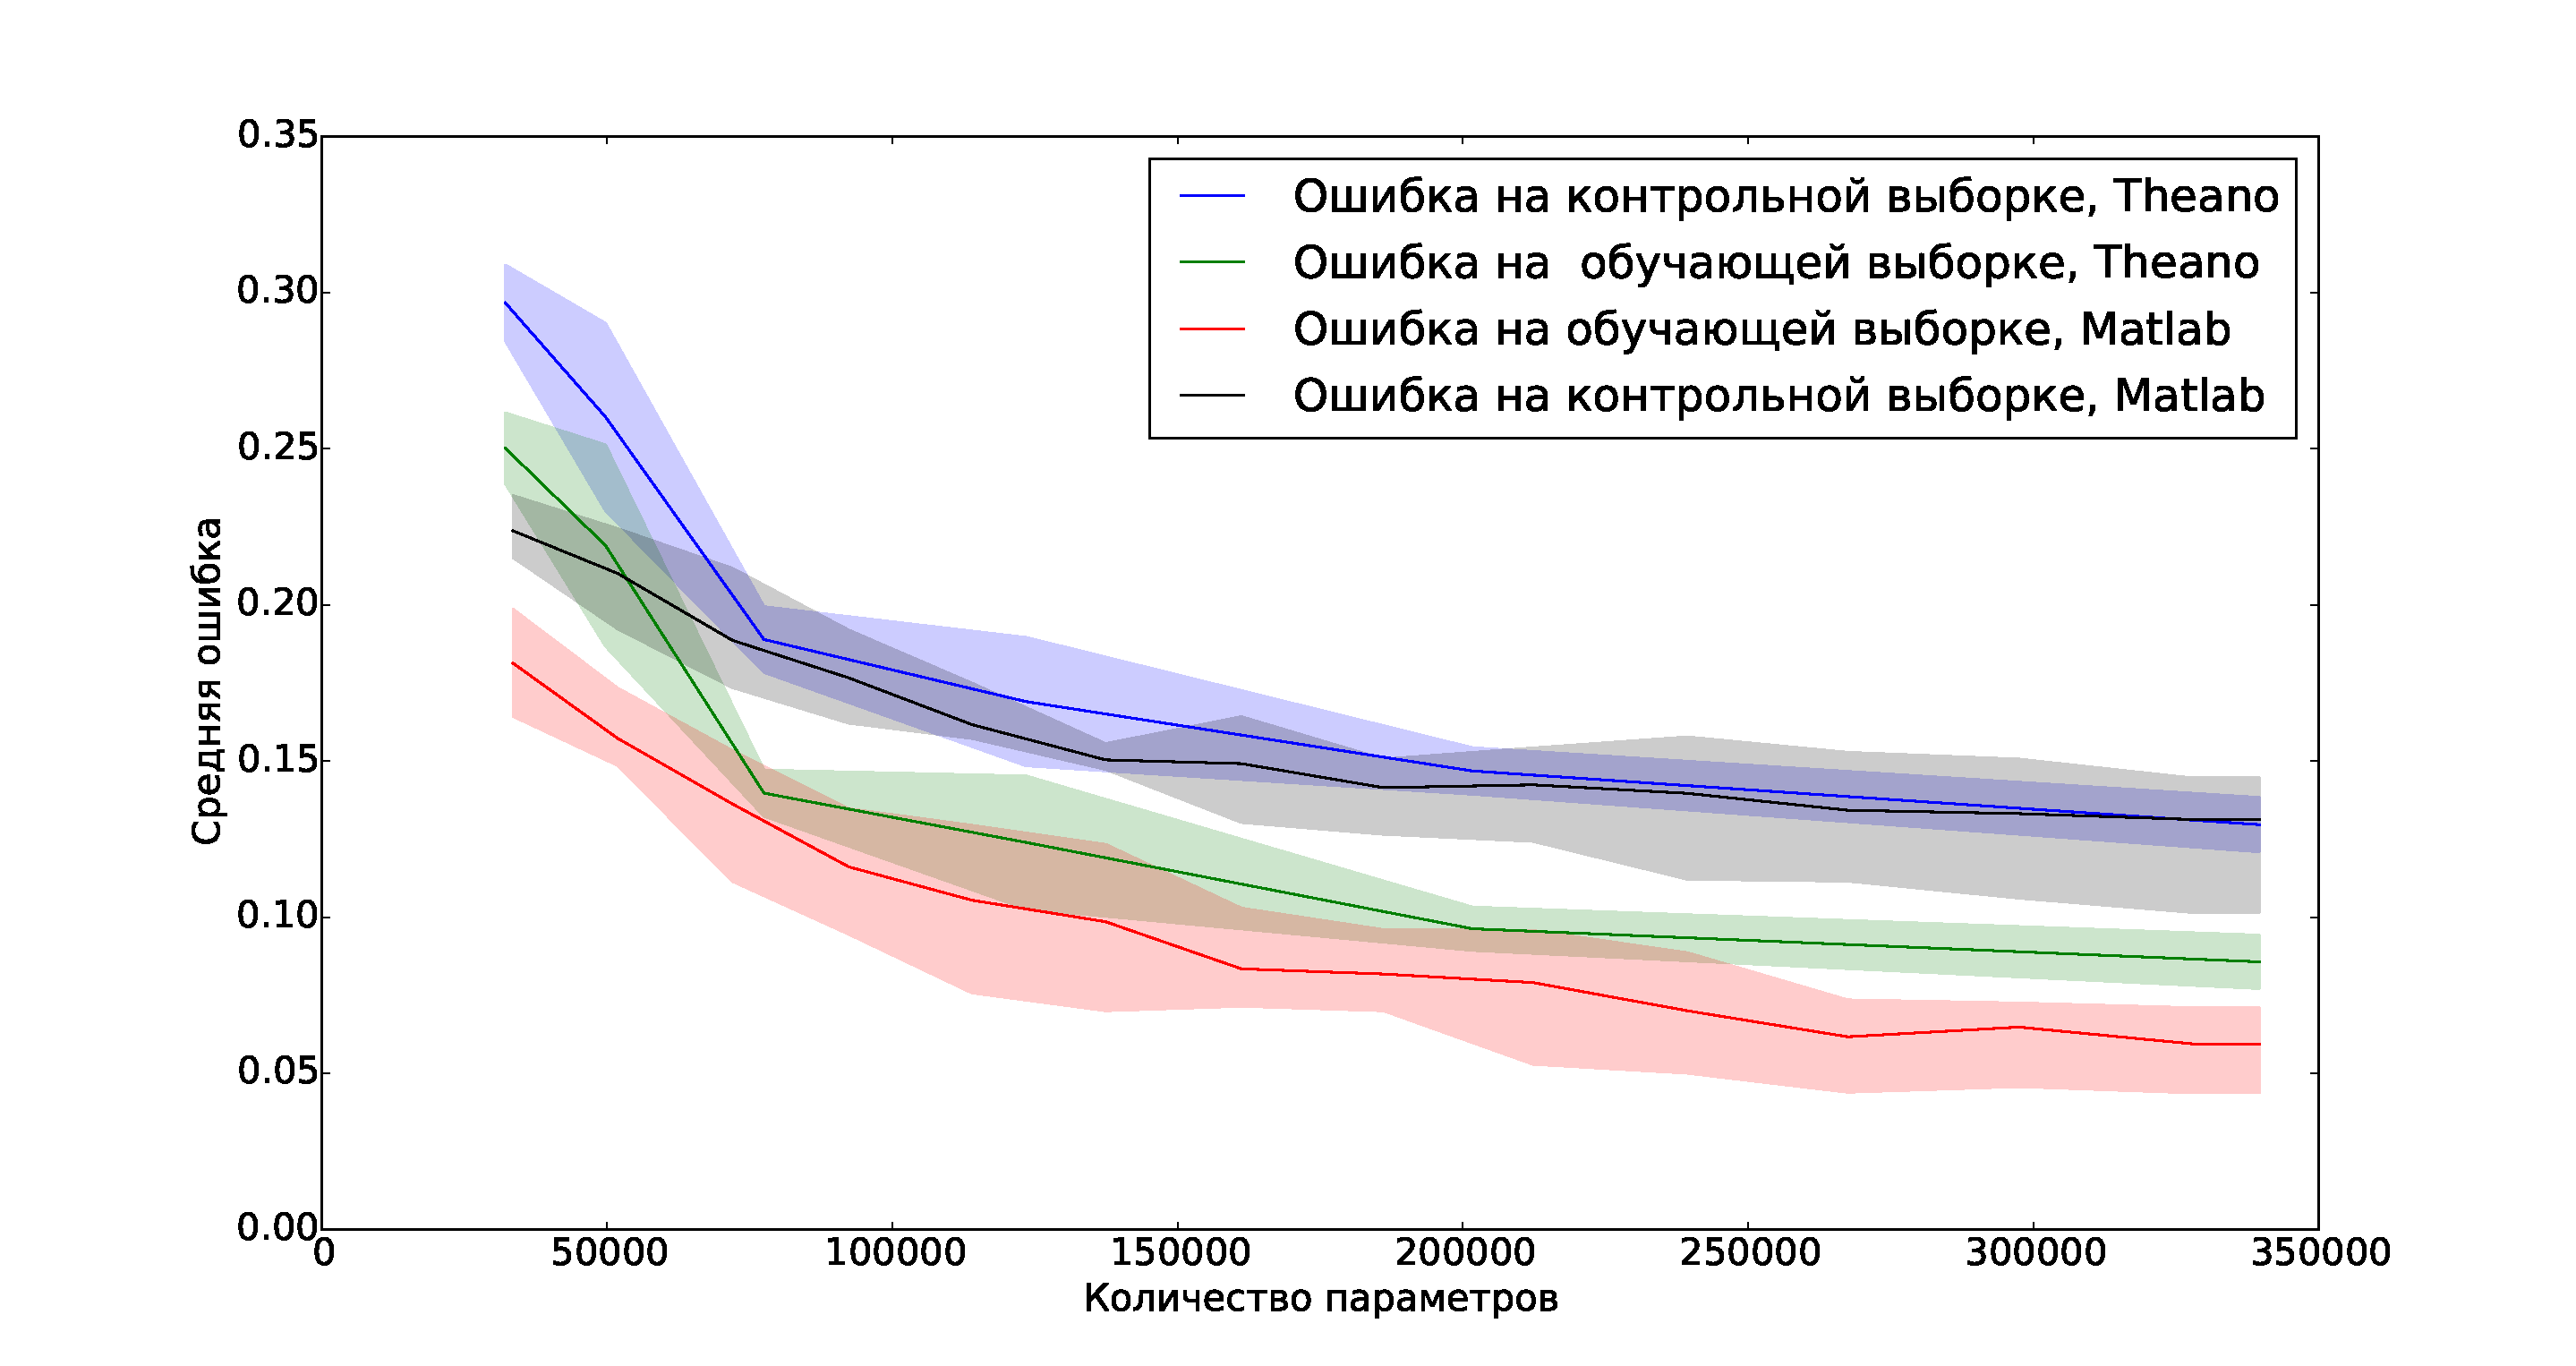
\includegraphics[width=1.0\textwidth]{plots/popova/neurons.pdf}
 \caption{Зависимость ошибки от числа нейронов}
 \label{fig:neurons}
\end{figure}


Для оценки зависимости качества классификации от размера обучающей выборки была проведена кросс-валидация с фиксированным количеством объектов в обучающей выборке (25\% исходной выборки) и переменным размером обучающей выборки. Число нейронов было установлено как 364:224:112. При проведении процедуры скользящего контроля для каждого отсчета было произведено пять запусков. График зависимости ошибки классификации от размера обучающей выборки представлен на рис.~\ref{fig:samples}.


\begin{figure}[tb!]
 \centering
  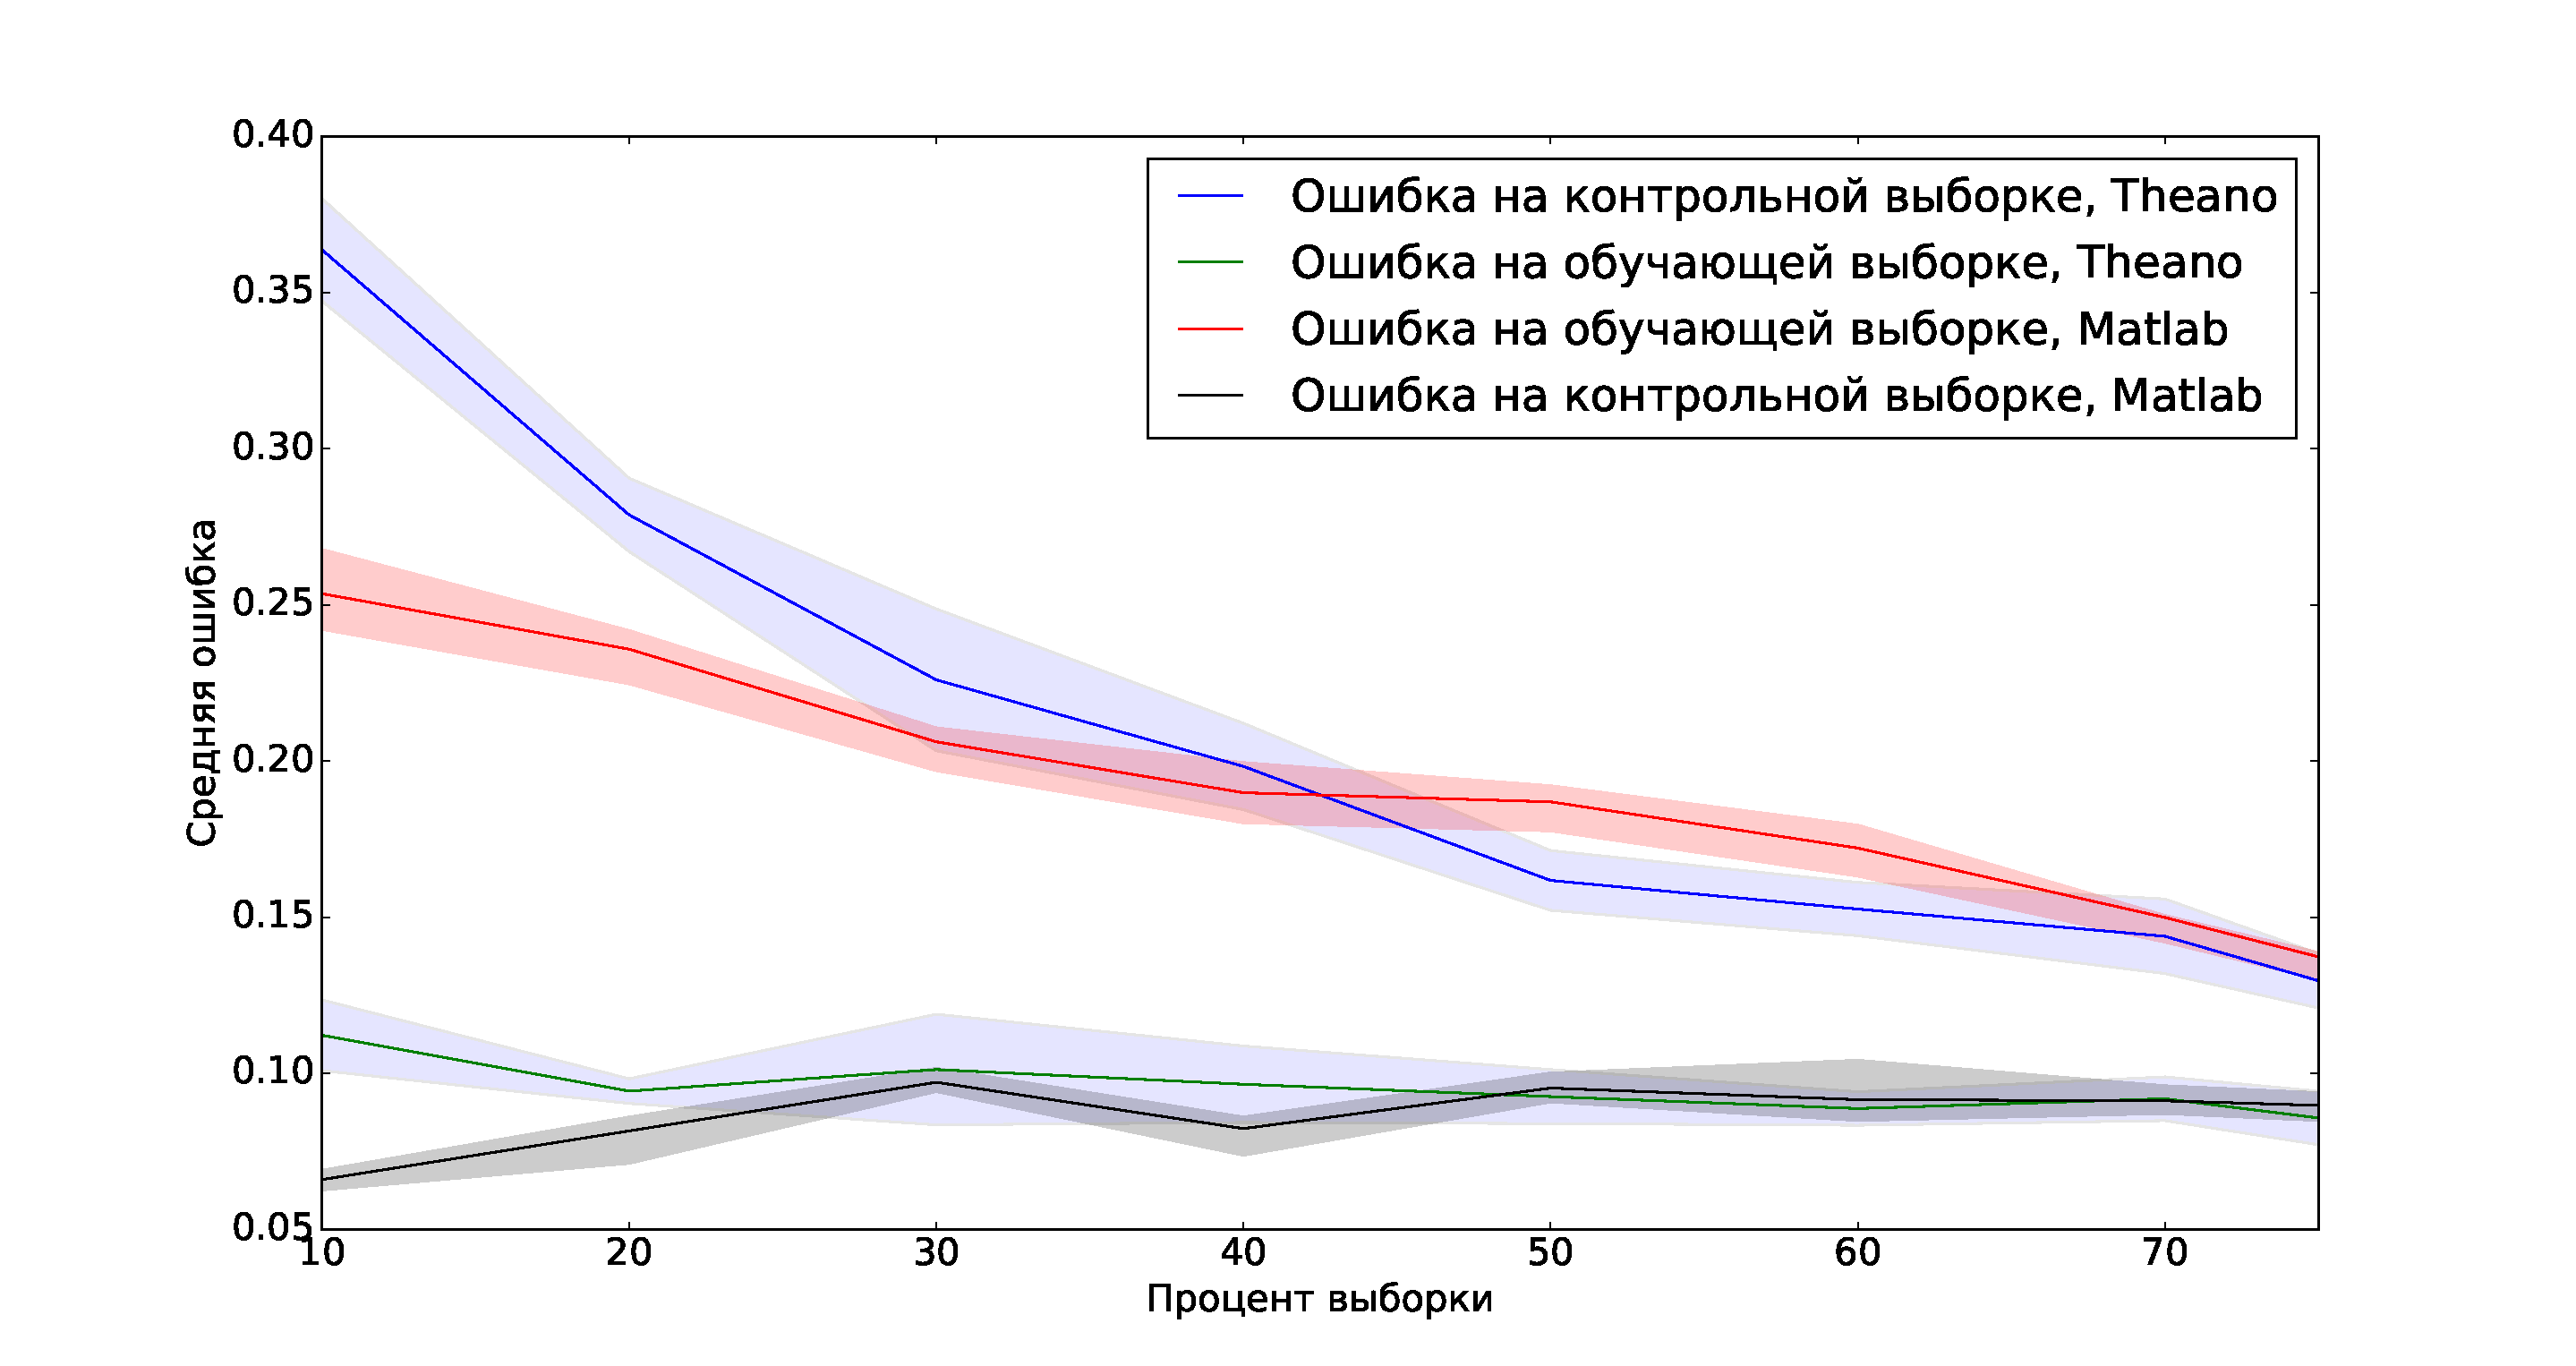
\includegraphics[width=1.0\textwidth]{plots/popova/samples.pdf}
 \caption{Зависимость ошибки от размера обучающей выборки}
 \label{fig:samples}
\end{figure}


Для исследования скорости оптимизации нейросети в зависимости от конфигурации Theano был сделан следующий эксперимент:
проводилось обучение двуслойной нейросети на основе подсчитанных заранее параметров ограниченной машины Больцмана~\eqref{eq:rbm} и автокодировщика~\eqref{eq:ae}. Обучение проходило за 100 итераций. При обучении алгоритм запускался параллельно с $r$ разными стартовыми позициями, $r \in \{1,\dots,4\}.$ Число нейронов было установлено как 300:200:100.
Запуск осуществлялся со следующими конфигурациями Theano:
\begin{itemize}
\item вычисление на центральном процессоре, задействовано
одно ядро;
\item вычисление на центральном процессоре, задействовано четыре ядра;
\item вычисление на центральном процессоре, задействовано восемь ядер;
\item вычисление на графическом процессоре.
\end{itemize}

Результаты эксперимента приведены на рис.~\ref{fig:speed}. Как видно из графика, вычисление с использованием CUDA показывает значительное ускорение по сравнению с вычислением на центральном процессоре.

\begin{figure}[tb!]
 \centering
  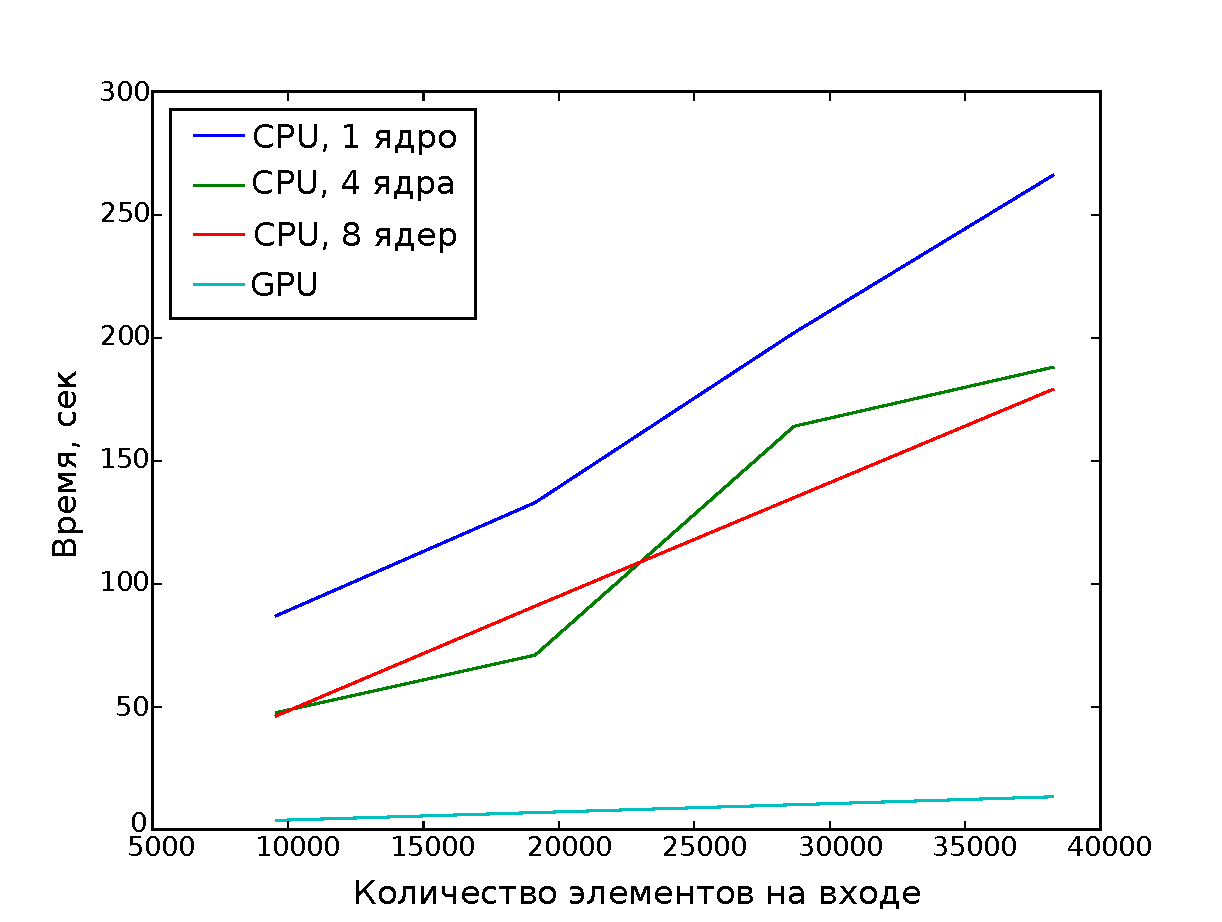
\includegraphics[width=0.8\textwidth]{plots/popova/result.pdf}
 \caption{Результаты эксперимента по исследованию скорости процесса обучения}
 \label{fig:speed}
\end{figure}

























\section{Выбор модели обнаружения перефраза в тексте}
В данном разделе решается задача выбора оптимальной нейросетевой модели  из класса рекуррентных нейронных сетей. Рекуррентной нейросетью называется нейросеть со связью между нейронами одного слоя. В качестве критерия оптимальности используется нижняя оценка правдоподобия модели. 

Для построения модели рекуррентной сети рассматривается модель из~\cite{sanborn}, решающая задачу определения сходства предложений.
Модель принимает на вход векторизованные представления слов. Векторизация выполняется с помощью алгоритма GloVe~\cite{glove}, основанного на факторизации матрицы слов-контекстов и использовании весовой функции для уменьшения значимости редких слов. Альтернативой этому алгоритму выступает линейная модель Word2vec, комбинирующая в себе Continuous Bag-of-Words, skip-gram, negative sampling~\cite{word2vec}. Несмотря на разные подходы к проблеме, GloVe и Word2vec оптимизируют схожие функционалы. Упрощенной линейной моделью Word2vec, предназначенной для классификации документов, является fastText --- метод, работающий на символьных $n$-граммах~\cite{fasttext}. 

Для решения задач, связанных с обработкой естественного языка применяются модели рекуррентных сетей(TODO). Обобщением рекуррентных моделей являются рекурсивные модели автокодировщиков, агрегирующие информацию от  входного текста не рекуррентно, а по дереву синтаксического разбора.

Предлагается подход, основанный на получении вариационной нижней оценки правдоподобия модели. Предлагаемый подход сравнивается с методом удаления параметров Optimal Brain Damage, базирующимся на анализе функции ошибки~\eqref{eq:obd}. 

Вычислительный эксперимент проводится на выборке размеченных пар предложений SemEval 2015. Для каждой пары предложений из корпуса дана экспертная оценка их семантической близости. Требуется построить модель, оценивающую семантическую близость двух предложений. Проблема рассматривается как задача многоклассовой классификации, аналогично~\cite{sanborn}. Критерием качества служит $F_1$-мера, учитывающая как полноту, так и точность предсказаний.
В качестве базовой модели рассматривается пара соединенных рекуррентных сетей с общим вектором параметров и softmax-классификатором на выходе.

\textbf{Постаноквка задачи. }
Для построения выборки используем набор пар предложений SemEval 2015~\cite{semeval2015}.
Каждому слову сопоставим вектор размерности $n$.
Обозначим через $l$ число слов в самом длинном предложении. Предложения длины, меньше $l$, дополним нулевыми векторами. 
Построим выборку
$$ \DD = \{(\bx_i,y_i)\}, i = 1,\dots,m,$$
где $\bx_i = [\bx_i^1,\bx_i^2]$ --- пары последовательностей векторов слов, соответствующих $i$-й паре предложений, $\bx_i^1, \bx_i^2 \in \RR^{n\times l}$;
$y_i \in \mathbb{Y} = \{0,\dots,R\}$ --- экспертная оценка семантической близости. 

Требуется построить модель $f(\bw): \RR^{n\times l} \times \RR^{n\times l} \to \mathbb{Y}$, сопоставляющую паре предложений $\bx_i^1$ и $\bx_i^2$ класс семантической близости, где $\bw \in \WW\subseteq\RR^s$ --- пространство параметров модели.
%$f: \RR^{n\times l} \times \RR^{n\times l} \times \WW \to Y$
Искомая модель выбирается из множества $M$ рекуррентных нейронных сетей с функцией активации $\tanh$. Модель 
\[
f(\bw): \RR^{n\times l} \times \RR^{n\times l} \to \mathbb{Y}
\]
%w,u,v
принадлежит искомому множеству моделей~$M$, если существуют такие матрицы перехода $\mathbf{w}_1\in \RR^{n\times m}, \mathbf{w}_2\in \RR^{n\times n}, \mathbf{w}_3\in \RR^{(Z \times 2n)}$ и вектор смещения $\bb \in \RR^{n}$, что для $j$-х элементов $\bx_{ij}^1, \bx_{ij}^2 \in \RR^m$ последовательностей $\bx_i^1$ и $\bx_i^2$ определены векторы скрытого слоя $\bh_{ij}^1, \bh_{ij}^2 \in \RR^{n}$:
\begin{gather}
\bh_{ij}^1 = \tanh(\mathbf{w}_1\cdot \bx_{ij}^1 + \mathbf{w}_2\cdot \bh_{i,j-1}^1 + \bb),\\
\bh_{ij}^2 = \tanh(\mathbf{w}_1\cdot \bx_{ij}^2 + \mathbf{w}_2\cdot \bh_{i,j-1}^2 + \bb).
\end{gather}

Для определения класса семантической близости используются последние значения скрытого слоя $\bh_{il}^1$ и $\bh_{il}^2$, объединенные в один вектор. После $l$-й итерации 
пару предложений будем относить к классу с наибольшим значением, полученным после $l$-й итерации, $j=1,\dots,l$:
\begin{gather}
y = \argmax_{c\in \{1,\dots,R\}}
\left(\mathbf{w}_3%\cdot
\begin{bmatrix}
\bh_{il}^1\\
\bh_{il}^2
\end{bmatrix}\right)[c],
\label{eq:classify}
\end{gather}
где $(\cdot)[c]$ --- $c$-я компонента вектора. 

В качестве оптимизируемой функции потерь $L$ выступает вариационная оценка правдоподобия модели~\eqref{eq:var_elbo}:
\begin{equation}
\label{eq:applied_elbo}
    L = -\sum_{i=1}^m \text{log}~p({y}_i|\mathbf{x}_i, \hat{\mathbf{w}}) + D_\text{KL}\bigl(q (\mathbf{w}) || p (\mathbf{w}|\mathbf{h})\bigr),\quad \hat{\mathbf{w}} \sim q,
\end{equation}
где $q$ --- вариацинное распределение, аппроксимирующее неизвестное апостериорное распределение параметров.
В качестве вариационного распределения выберем нормальное распределение:
$$q \sim \NNN(\boldsymbol{\mu}_q,\mathbf{A}_q^{-1}),$$
где $\boldsymbol{\mu}_q,\mathbf{A}_q^{-1}$ --- вектор средних и матрица ковариации.
Априорное распределение $\PP(\bw|\bbf)$ вектора параметров $\bw$ будем считать нормальным с параметрами $\boldsymbol{\mu}$ и $\mathbf{A}$:
$$\PP(\bw|\mathbf{h}) \sim \NNN(\boldsymbol{\mu}, \mathbf{A}^{-1}),$$
где $\boldsymbol{\mu}$ --- вектор средних, $\mathbf{A}^{-1}$ --- матрица ковариаций.

Рассмотрим частные случаи вида матриц ковариаций $\mathbf{A}^{-1}_q$ и $\mathbf{A}^{-1}$. Так как априори нет предпочтений при выборе параметров, то априорное распределение для всех параметров считаем одинаковым, т. е. вектор средних $\boldsymbol{\mu} = \mu$, матрица ковариаций скалярна: $\mathbf{A}^{-1} = \alpha\II$.

Априорное распределение уточняется после каждого шага оптимизации вариационных параметров.
Алгоритм решения оптимизационной задачи заключается в выполнении градиентного шага при заданном априорном распределении, вычислении апостериорного распределения и аппроксимации нового априорного распределения полученным апостериорным.

Рассмотрим различные виды матрицы ковариаций $\mathbf{A}^{-1}_q$ вариационного распределения $q$.
\begin{enumerate}
	\item Матрица ковариаций скалярна: $\mathbf{A}^{-1}_q = \alpha_q\II$.
	В этом случае дивергенция выглядит следующим образом:$$
	\DKL\bigl(\NNN(\boldsymbol{\mu}_q,\mathbf{A}^{-1}_q||\bmupr,\mathbf{A}^{-1}))\bigr) = \sum\limits_{i=1}^{|\mathbf{W}|}\big(\log\frac{\alpha}{\alpha_q} + \frac{(\mu-\mu_{q}[i])^2 + \alpha_q^2 + \alpha^2}{2\alpha^2}\big),
	$$
где $\mu_{q}[i]$ --- $i$-я компонента вектора $\boldsymbol{\mu_q}$.

	По значениям параметров $\alpha_q$ и $\boldsymbol{\mu}_q$ вариационного распределения  вычислим оптимальные параметры априорного. Из условия $$\frac\partial{\partial\mu}\DKL = \sum_{i=1}^{|\mathbf{W}|}\frac{\mu-\mu_{q}[i]}{\alpha^2}=0$$ получаем выражения для $\mu$ на следующей итерации $${\mu}' = \frac{1}{|\mathbf{W}|}\sum_{i=1}^{|\mathbf{W}|} \mu_{q}[i]$$.
	Аналогично $$\frac\partial{\partial \alpha^2}\DKL = \sum_{i=1}^{|\mathbf{W}|} \frac1{2\alpha^2}-\frac{(\mu-\mu_{q}[i])^2 + \alpha_q^2}{2\alpha^4}=0 \ \Rightarrow \ \hat{\alpha}^2 = \frac{1}{|\mathbf{W}|}\sum_{i=1}^{|\mathbf{W}|} (\mu-{\mu_{q}[i]})^2 + \alpha_q^2.$$

	\item Матрица ковариаций диагональна: $\mathbf{A}^{-1}_q = \text{diag}(\boldsymbol{\alpha}_q^2)$.	

	В этом случае \[\DKL\bigl(\NNN(\boldsymbol{\mu}_q,\mathbf{A}^{-1}_q||\bmupr,\mathbf{A}^{-1}))\bigr)  = \sum\limits_{i=1}^{|\mathbf{W}|}(\log\frac{a}{\alpha[i]} + \frac{(\mu-\mu_{q}[i])^2 + \sigma[i]^2 + \sigma^2}{2\sigma^2}).\]
	Значения параметров априорного распределения для следующей итерации вычисляются следующим образом:
\[ \text{из} \ \frac\partial{\partial\mu}\DKL = \sum\limits_{i=1}^{|\mathbf{W}|}\frac{\mu-\mu_{q}[i]}{\alpha^2}=0 \ \text{получаем} \ \hat{\mu} = \frac{1}{|\mathbf{W}|}\sum\limits_{i=1}^{|\mathbf{W}|} \mu_{q}[i],\]
\[ \text{из} \ \frac\partial{\partial a^2}\DKL = \sum\limits_{i=1}^{|\mathbf{W}|} \frac1{2\alpha^2}-\frac{(\mu-\mu_{q}[i])^2 + \alpha[i]^2}{2\alpha^4}=0 \ \text{получаем} \ \hat{\alpha}^2 = \frac{1}{|\mathbf{W}|}\sum\limits_{i=1}^{|\mathbf{W}|} (\mu-\mu_{q}[i])^2 + \alpha[i]^2.\]
\end{enumerate}


Оптимизация параметров сводится к следующему алгоритму:\\
\begin{enumerate}
\item Инициализировать~$\mathbf{a}_q = \textbf{1}, \ \boldsymbol{\mu}_q = \textbf{0}, {\mu} = 0, \ \alpha^2 = 1$.\\
{\textbf{Повторять}}:\\
\item Сделать градиентный шаг~\eqref{eq:sgd} по вариационным параметрам $\boldsymbol{\theta} = [\boldsymbol{mu}, \boldsymbol{\alpha}_q]$.
\item Обновить параметры априорного распределения.\\
\item {\textbf{Пока}} значение $L$ не стабилизируется.
\end{enumerate}

\textbf{Удаление нерелевантных параметров}
Введем множество индексов активных параметров модели $\mathcal{A} = \{i | w[i] \neq 0\} $. Для увеличения правдоподобия модели предлагается уменьшить число активных параметров $|\mathcal{A}|$. Для удаления выберем параметры, имеющие наибольшую плотность вариационной вероятности $\rho$ в нуле.
Если апостериорная матрица ковариаций скалярна, то  
\begin{gather}
\rho_i = \exp\left(-\frac{\mu_{q}[i]^2}{\alpha_{q}[i]^2}\right).
\end{gather}
Чем больше $\rho$, тем меньше $|\frac{\mu_{q}[i]}{\alpha_{q}[i]}|$, поэтому удаляются параметры со значением $|\frac{\mu_{q}[i]}{\alpha_{q}[i]}| < \lambda$, где $\lambda$ --- пороговое значение. Варьируя пороговое значение $\lambda$, выбираем оптимальное число неудаленных параметров.
Для диагонального вида матрицы ковариаций критерий удаления параметров записывается как $|\frac{\mu_{q}[i]}{\alpha_{q}[i]}| < \lambda$.

\textbf{Вычислительный эксперимент. }
Цель эксперимента~--- проверка работоспособности предложенного алгоритма и сравнение результатов с ранее полученными. В качестве данных использовалась выборка SemEval 2015, состоящая из 8331 пары схожих и несхожих предложений. Слова преобразовывались в векторы размерности 50 при помощи алгоритма GloVe~\cite{glove}.

Для базовых алгоритмов тренировочная, валидационная и тестовая выборки составили 70\%, 15\% и 15\% соответственно.
Для рекуррентной нейронной сети, полученной вариационным методом, валидационная выборка отсутствовала, а тренировочная и тестовая выборки составили 85\% и 15\% соответственно.
Критерием качества была выбрана $F_1$-мера.
В качестве базовых алгоритмов использовались линейная регрессия, метод ближайших соседей, решающее дерево и модификация метода опорных векторов SVC. Базовые алгоритмы взяты из библиотеки sklearn~\cite{sklearn}. 
Дополнительно были построены рекуррентная нейросеть с одним скрытым слоем~\cite{sanborn} и нейросеть с одним скрытым слоем и вариационной оптимизацией параметров.


\begin{figure}[!h]
	\centering
	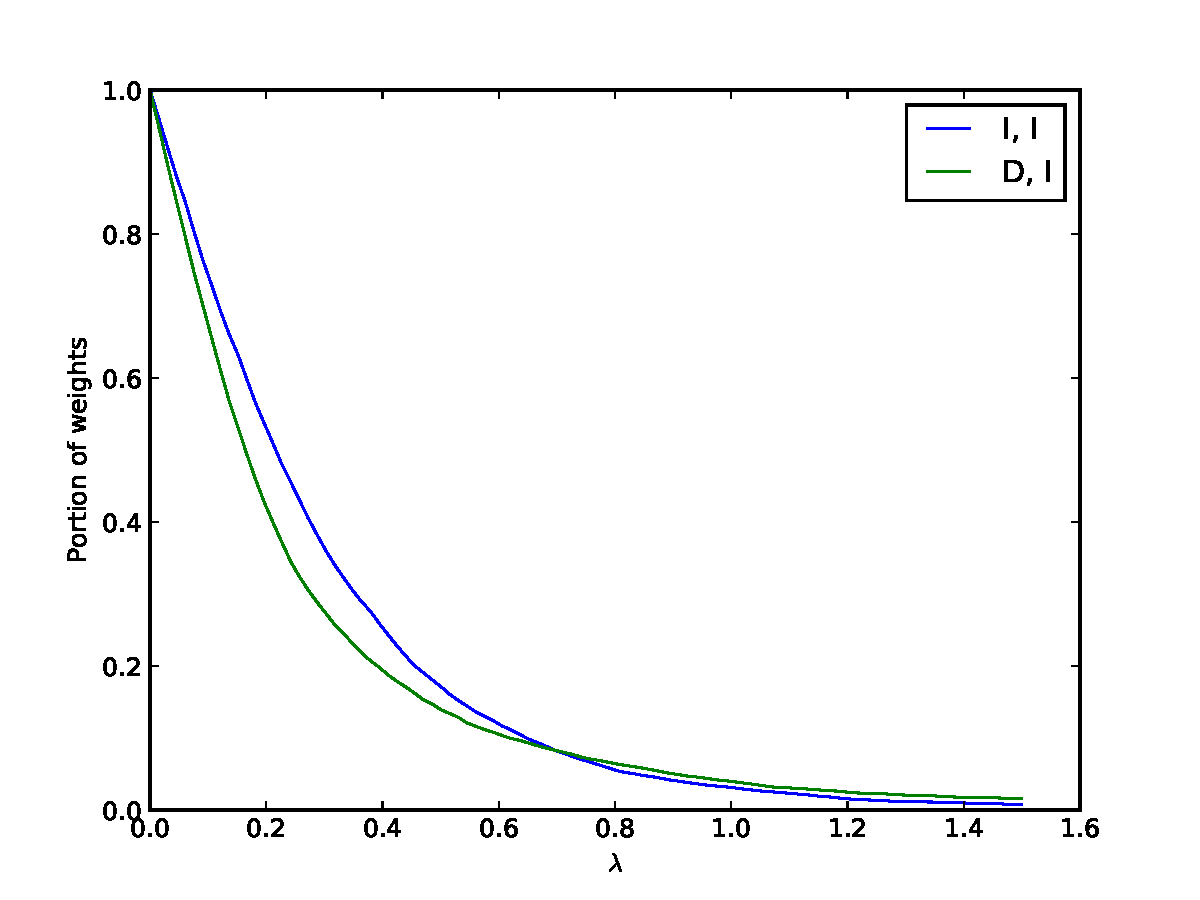
\includegraphics[width=0.5\textwidth]{plots/smerdov/lambdas.pdf}
	\caption{Доля неудаленных параметров сети в зависимости от порогового значения $\lambda$ для скалярного~($I$) и диагонального~($D$) вида апостериорной матрицы ковариаций.}
	\label{lambdas}
\end{figure}

 

На рис.~\ref{evidence_I_I} и~\ref{evidence_I_D} представлена зависимость оценки правдоподобия $L$ \eqref{eq:applied_elbo} от параметра $\lambda$.
Для обоих случаев существует оптимальное значение $\lambda$, минимизирующее $L$; модели с таким параметром будут оптимальными. На рис.~\ref{score_I_I},~\ref{score_I_D},~\ref{portion_I_I} и~\ref{portion_I_D} отображены зависимости качества модели от $\lambda$ и доли выброшенных параметров. Видно, что даже при удалении большинства параметров из сети качество предсказаний меняется несущественно, что говорит о слишком большом числе параметров исходной модели.

Из рис.~\ref{lambdas} видно, что при малых $\lambda$ из сети с диагональной апостериорной матрицей ковариаций удаляется больше весов, а при больших $\lambda$ --- меньше, что говорит о лучшем отборе параметров такой моделью.


\begin{table}[!htp]
	\centering
	\caption{Результаты вычислительного эксперимента}
	\label{my-label}
	\begin{tabularx}{\textwidth}{|X|l|l|}
		\hline
		\bf Модель          & $F_1$, \bf валидация & $F_1$,\bf тест\\ \hline
		Логистическая регрессия   & 0,286                 & 0,286            \\ \hline
		SVC                    & 0,290                 & 0,290            \\ \hline
		Дерево решений & 0,316                 & 0,316            \\ \hline
		KNN   & 0,322                 & 0,322            \\ \hline
		Рекуррентная модель                    & 0,393                 & 0,362            \\ \hline
		Рекуррентная модель с вариационным распределением, $\mathbf{A} = \alpha\mathbf{I}, \mathbf{A}_q = \alpha_q\mathbf{I}$  &  ---                     & 0,311            \\ \hline
		Рекуррентная модель с вариационным распределением, $\mathbf{A} = \alpha\mathbf{I}, \mathbf{A}_q$ диагональная   &  ---                     & 0,330             \\ \hline
	\end{tabularx}
\end{table}


\begin{figure}[!htp]
%\begin{tabular}{>{\centering}m{6.7cm} c}
% Скалярная апостериорная матрица	& Диагональная апостериорная матрица \\ %\hline
%\end{tabular}
	\vspace{-1mm}
	\centering
	\begin{subfigure}[!tp]{0.45\textwidth}
%		Скалярная апостериорная матрица	
		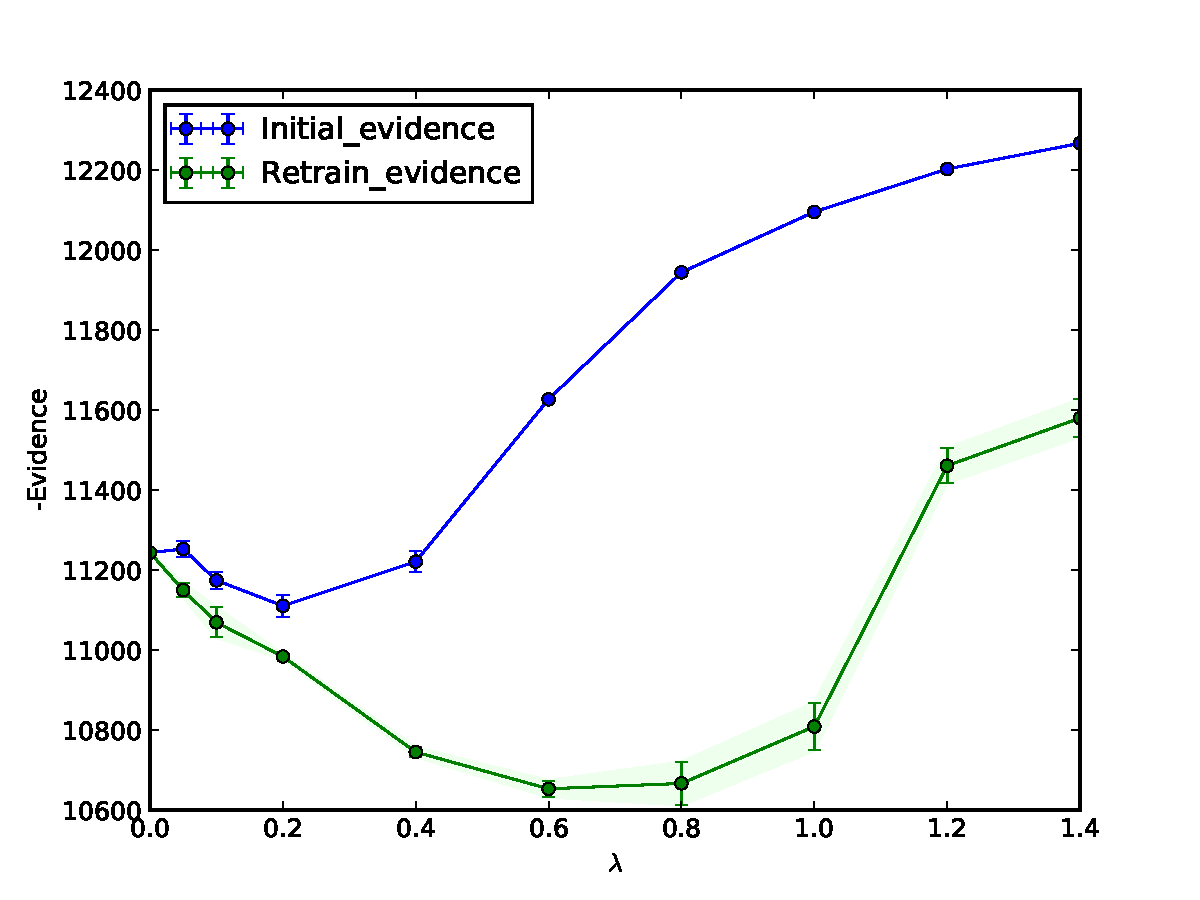
\includegraphics[width=\textwidth]{plots/smerdov/pruning_evidence_I_I.pdf}
		\caption{}
%		\caption{$L(\lambda)$, скалярная апостериорная матрица.}
		\label{evidence_I_I}
	\end{subfigure}
	\vspace{-1mm}
	~
	\hspace{-2mm}
	\begin{subfigure}[!htbp]{0.45\textwidth}
%	Диагональная апостериорная матрица 
		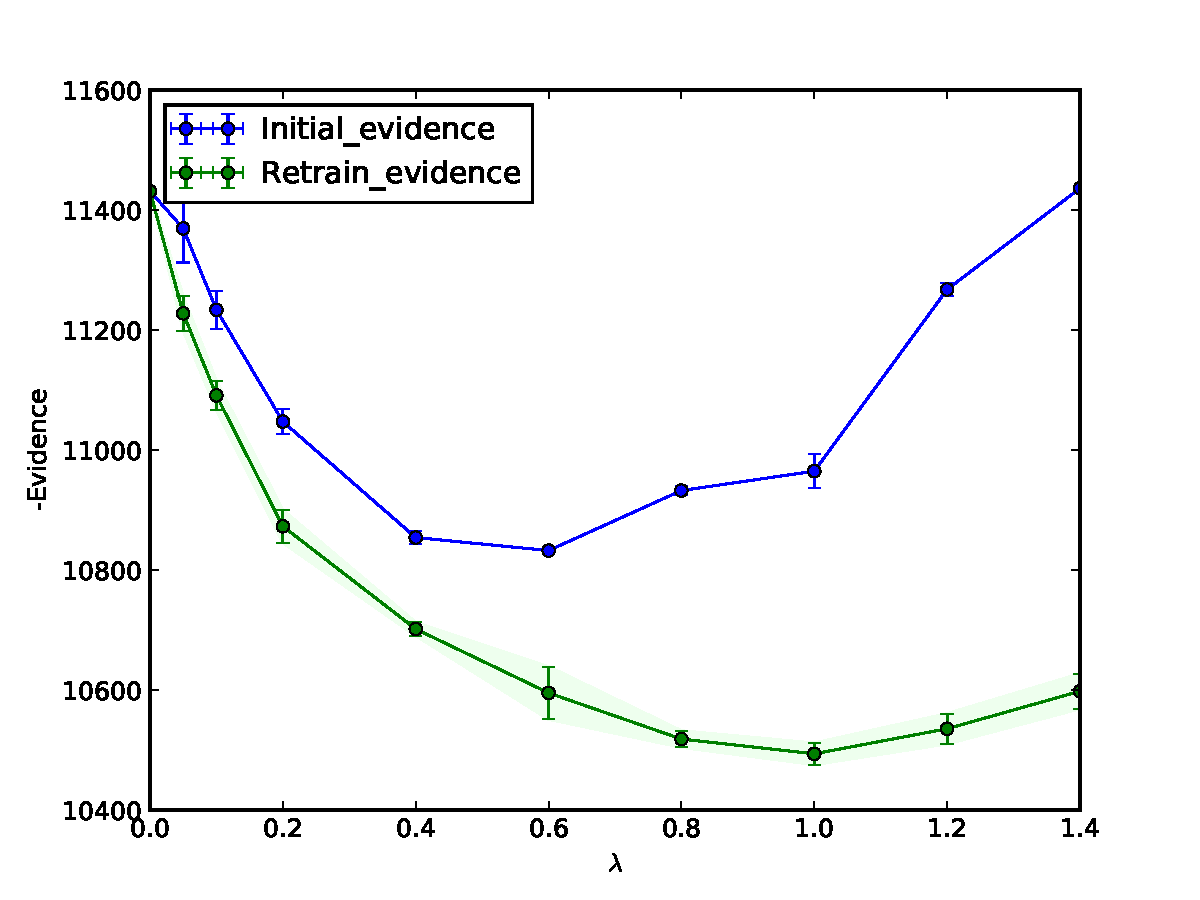
\includegraphics[width=\textwidth]{plots/smerdov/pruning_evidence_D_I.pdf}
%		\caption{$L(\lambda)$, диагональная апостериорная матрица.}
		\caption{}
		\label{evidence_I_D}
	\end{subfigure}
	\newline
	\vspace{-1mm}
	\begin{subfigure}[!htbp]{0.45\textwidth}
		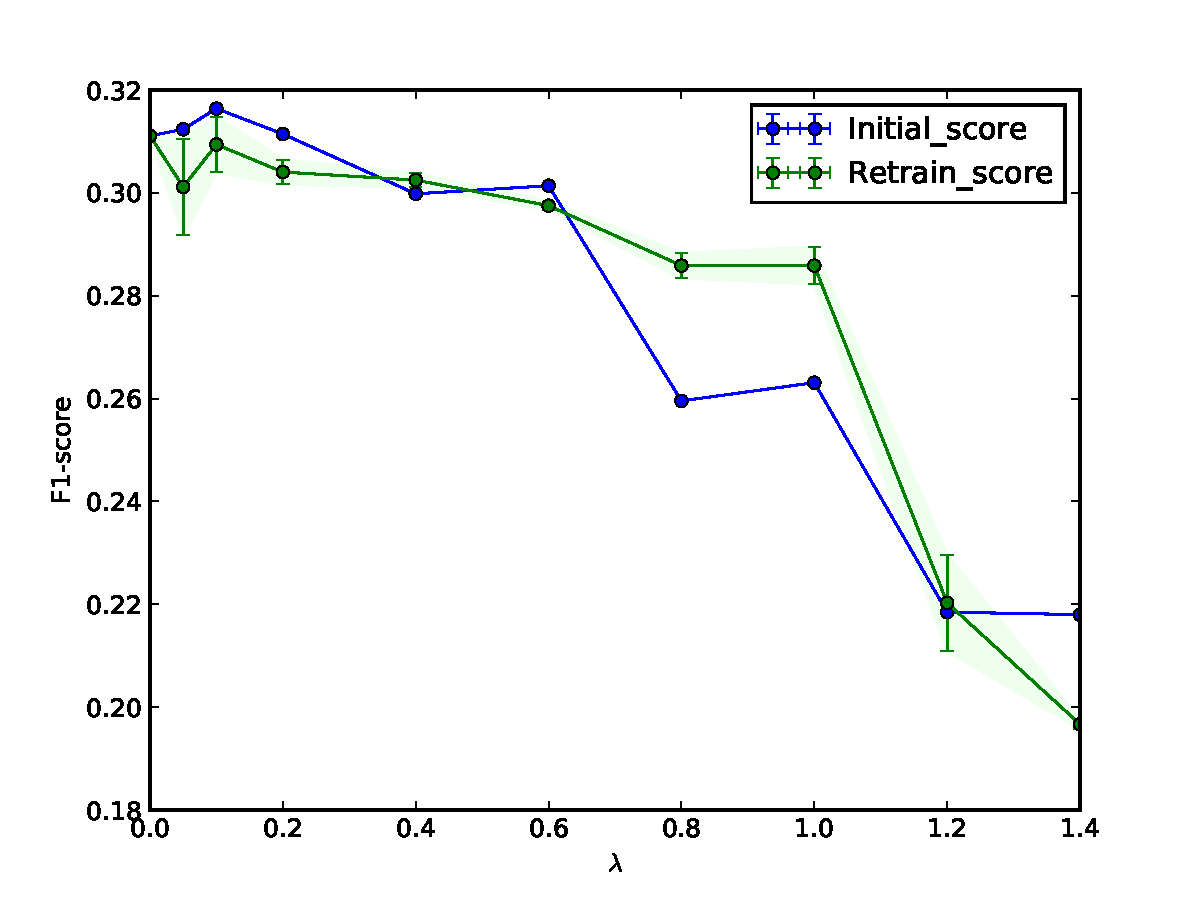
\includegraphics[width=\textwidth]{plots/smerdov/lambda_I_I.pdf}
%		\caption{F1-score($\lambda$), скалярная апостериорная матрица.}
		\caption{}
		\label{score_I_I}
	\end{subfigure}
%	\hspace{1mm}
	~
	\begin{subfigure}[!htbp]{0.45\textwidth}
		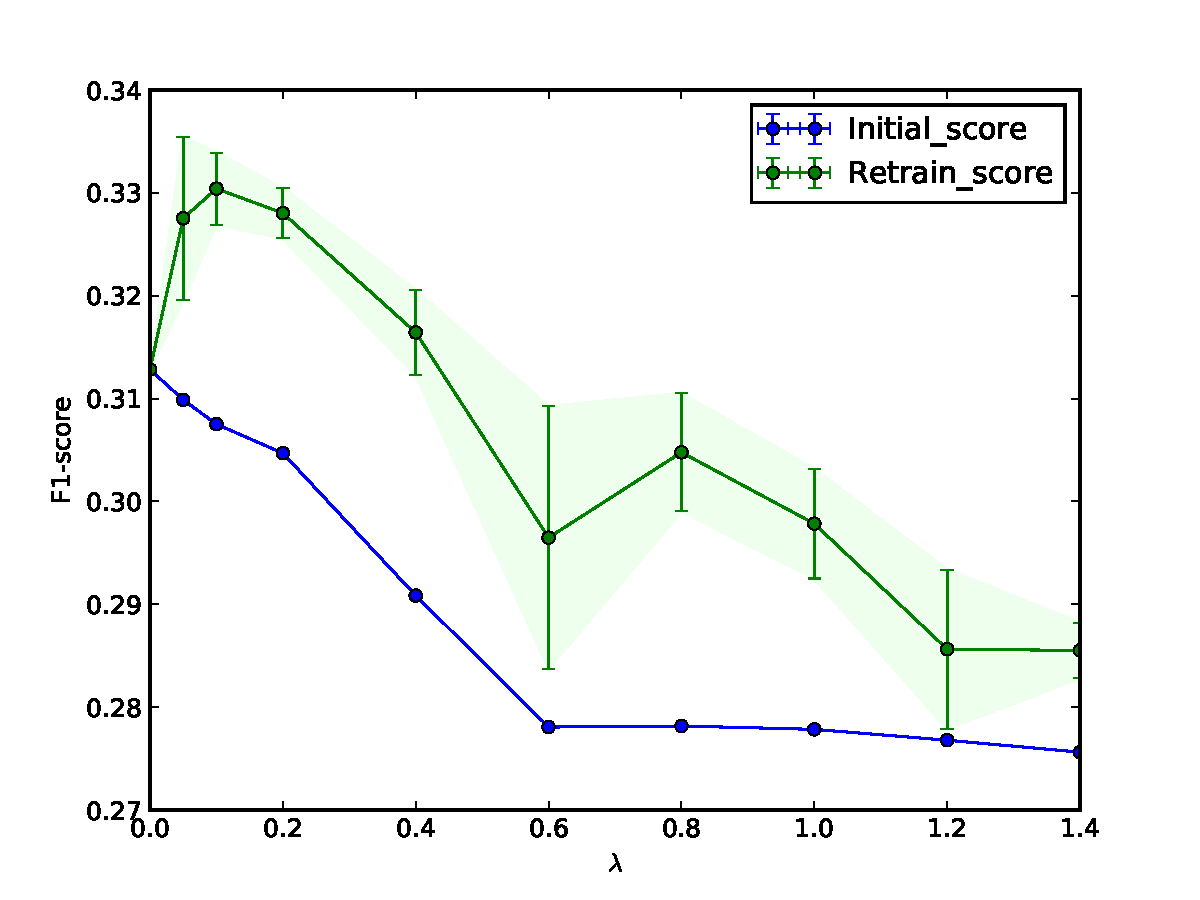
\includegraphics[width=\textwidth]{plots/smerdov/lambda_D_I.pdf}
%		\caption{F1-score($\lambda$), диагональная апостериорная матрица.}
		\caption{}
		\label{score_I_D}
	\end{subfigure}
	\newline
%	~
	\begin{subfigure}[!htbp]{0.45\textwidth}
		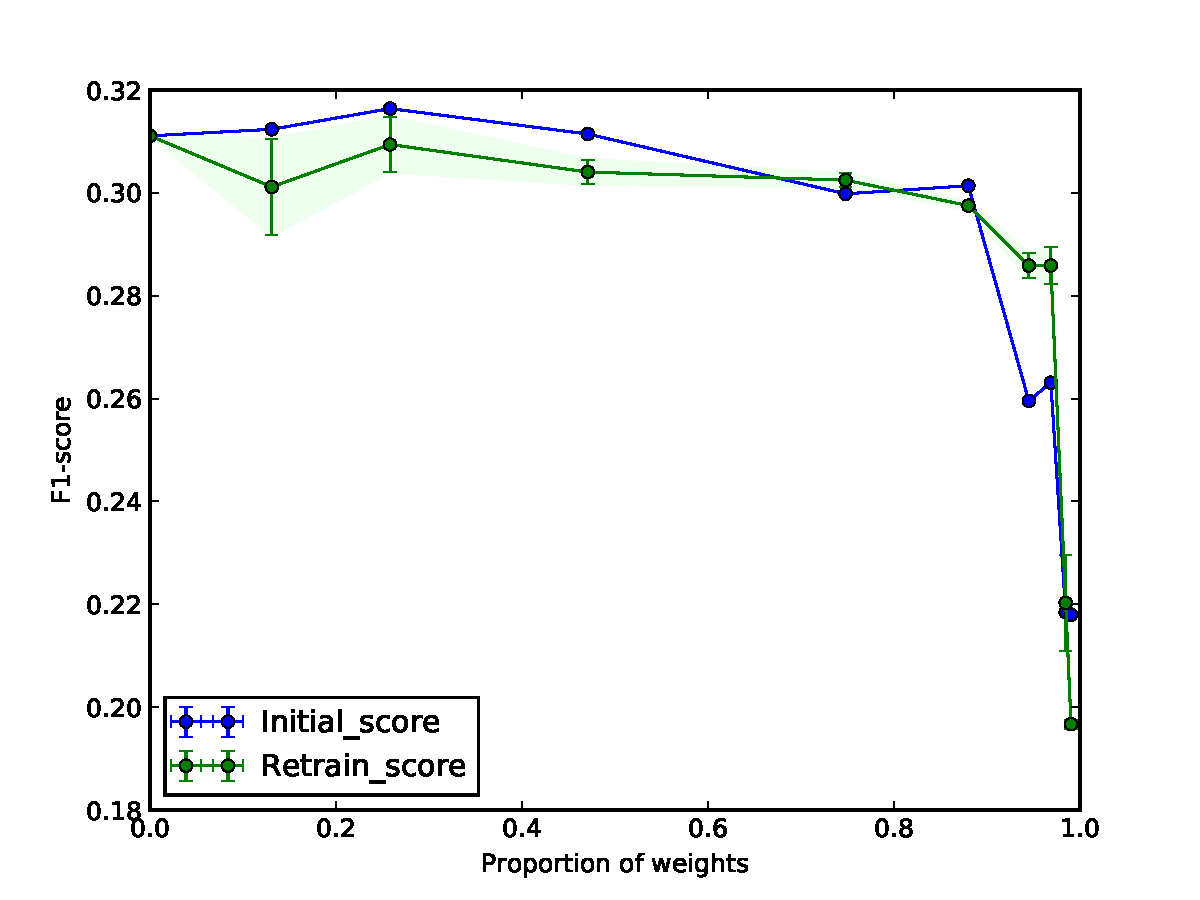
\includegraphics[width=\textwidth]{plots/smerdov/portion_I_I.pdf}
%		\caption{Зависимость качества от доли выброшенных параметров, скалярная апостериорная матрица.}
		\caption{}
		\label{portion_I_I}
	\end{subfigure}
%	\hspace{3mm}
	~
	\begin{subfigure}[!htbp]{0.45\textwidth}
		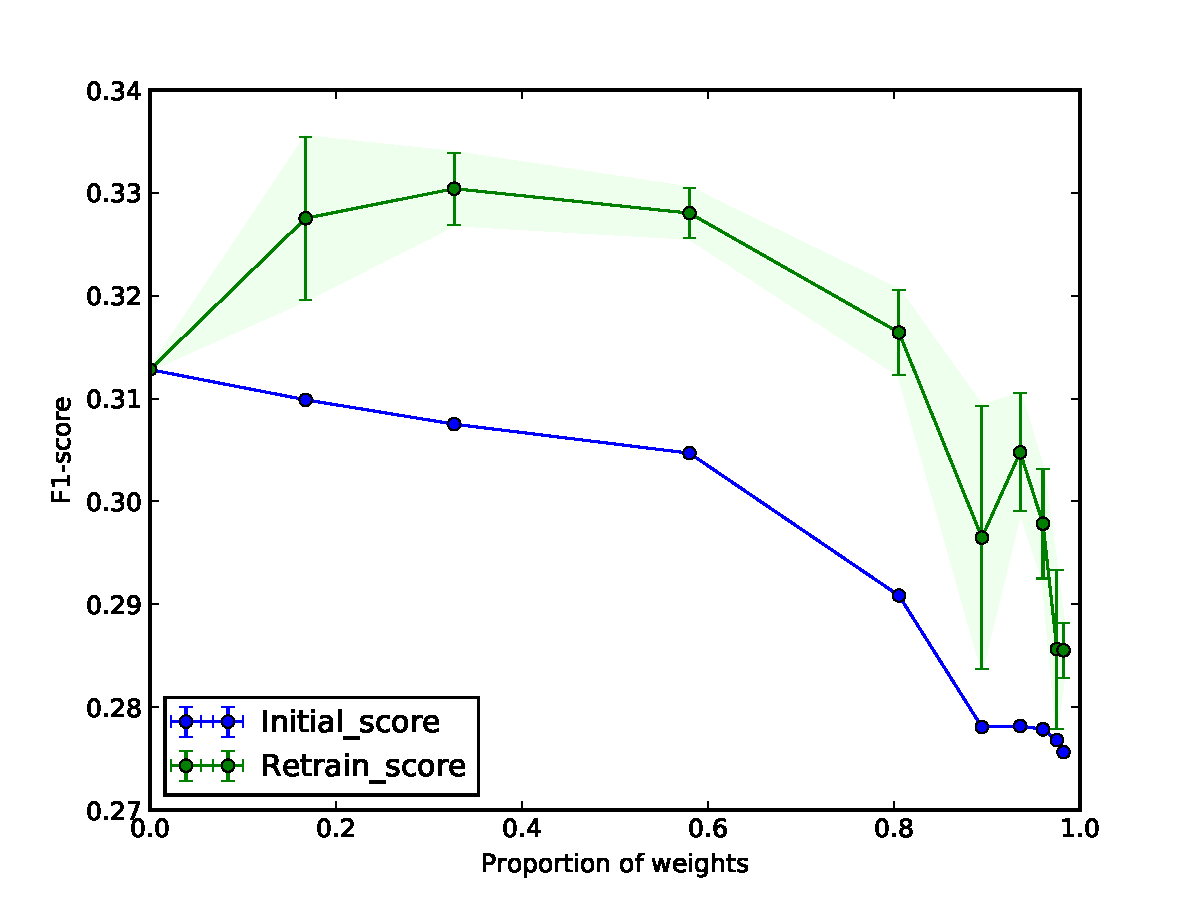
\includegraphics[width=\textwidth]{plots/smerdov/portion_D_I.pdf}
%		\caption{Зависимость качества от доли выброшенных параметров, диагональная апостериорная матрица.}
		\caption{}
		\label{portion_I_D}
	\end{subfigure}
	\hspace{1mm}
	\caption{Зависимость нижней оценки правдоподобия модели и F1-меры от $\lambda$} для скалярной (а, б, в) и диагональной(г, д, е) матриц.
	\label{results}
\end{figure}






























\section{Определение релевантности параметров модели глубокого обучения}
В данном разделе решается задача выбора субоптимальной структуры нейронной сети. Предлагается удалять наименее релевантные параметры модели. Под релевантностью~\cite{nips} подразумевается то, насколько параметр влияет на функцию ошибки. Малая релевантность указывает на то, что удаление этого параметра не влечет значимого изменения функции ошибки. Метод предлагает построение исходной избыточной сложности нейросети с большим числом избыточных параметров. Для определения релевантности параметров предлагается оптимизацировать параметры и гиперпараметры в единой процедуре. Для удаления параметров предлагается использовать метод Белсли~\cite{neychev} .

Проверка и анализ метода проводится на выборке Boston Housing, Wine и синтетических данных. Результат сравнивается с моделью, полученной при помощи базовых алгоритмов.

\textbf{Постановка задачи}

Задана выборка
$$\mathfrak{D} = \{\textbf{x}_i,y_i\},~ i =1,...,m$$
где~$\textbf{x}_i \in \mathbb{R}^{m}$,~$y_i \in \{1, \dots, R\}$,~$R$ --- число классов.
Рассмотрим модель~$$\mathbf{f}(\mathbf{x}, \mathbf{w}): \mathbb{R}^m \times \mathbb{W} \to [0,1]^R$$, где
$$\mathbf{f}((\mathbf{x}, \mathbf{w}) = \textbf{softmax}\bigl( f_1(f_2(...(f_{|V|}(\mathbf{x}, \mathbf{w})\bigr)$$.

Параметр~$w_j$ модели~$\mathbf{f}$  называется активным, если~$w_j \not = 0$. Множество индексов активных параметров обозначим~$\mathcal{A}$.
Задано пространство параметров модели:
$$\mathbb{W_\mathcal{A}} = \{ \textbf{w} \in \mathbb{W}|~w_j\not=0,~j \in \mathcal{A}  \}.$$


Для модели~$\mathbf{f}$ с множеством индексов активных параметров~$\mathcal{A}$ и соответствующего ей вектора параметров~$\textbf{w} \in \mathbb{W_\mathcal{A}}$  определим логарифмическую функцию правдоподобия выборки:
$$L = \log p(\mathbf{Y}|\mathbf{X}, \mathbf{w}, \mathcal{A}),$$
где~$p(\mathfrak{D}|\mathcal{A},\textbf{w})$ --- апостериорная вероятность выборки~$\mathfrak{D}$ при заданных~$\textbf{w}, \mathcal{A}$.

Аналогично~\eqref{eq:applied_elbo} будем проводить оптимизацию вариационной оценки правдоподобия модели, где в качестве вариационного распределения $q$ и априорного распределения параметров $p(\mathbf{w}|\mathbf{h})$ выступает нормальное.

TODO: не понял, спросить у Андрея.
\textbf{Случайное удаление. }
Метод случайного удаления заключается в том, что случайным образом удаляется некоторый параметр $w_\xi$ из множества активных параметров сети.  Индекс параметра $\xi$ из равномерного распределения  случайная величина, предположительно доставляющая оптимум в (2.11).
$$\xi \sim \mathcal{U}(\mathcal{A}). \eqno(3.1.1)$$

\textbf{Оптимальное прореживание. }
Метод оптимального прореживания \cite{cun1990} использует вторую производную целевой функции (2.4) по параметрам для определения нерелевантных параметров. Рассмотрим функцию потерь~$\mathcal{L}$ (2.4) разложенную в ряд Тейлора в некоторой окрестности вектора параметров~$\textbf{w}$:
$$\delta \mathcal{L} = \sum_{j\in \mathcal{A}} g_j\delta w_j + \frac{1}{2}\sum_{i,j\in \mathcal{A}} h_{ij}\delta w_i\delta w_j + O(||\delta\textbf{w}||^3), \eqno(3.2.1)$$
где~$\delta w_j~$ --- компоненты вектора~$\delta\textbf{w}$,~$g_j$ --- компоненты вектора градиента~$\nabla \mathcal{L}$, а~$h_{ij}$ --- компоненты гесcиана~$\textbf{H}$:
$$g_j = \frac{\partial \mathcal{L}}{\partial w_j}, \qquad h_{ij} = \frac{\partial^2\mathcal{L}}{\partial w_i \partial w_j}. \eqno(3.2.2)$$

Задача является вычислительно сложной в силу высокой размерности матрицы \textbf{H}. Введем предположение \cite{cun1990}, о том что удаление нескольких параметров приводит к такому же изменению функции потерь~$\mathcal{L}$, как и суммарное изменение при индивидуальном удалении:
$$\delta \mathcal{L} = \sum_{j\in \mathcal{A}} \delta \mathcal{L}_j, \eqno(3.2.3)$$
где~$\mathcal{A}$ --- множество активных параметров,~$\delta\mathcal{L}_j$ --- изменение функции потерь при удалении одного параметра~$\textbf{w}_j$.

В силу данного предположения будем рассматривать только диагональные элементы матрицы \textbf{H}. После введенного предположения, выражение (3.2.1) принимает вид
$$\delta \mathcal{L} = \frac{1}{2} \sum_{j\in \mathcal{A}} h_{jj}\delta w_j^2, \eqno(3.2.4)$$

Получаем следующую задачу оптимизации:

$$\xi = \argmin_{j\in \mathcal{A}} h_{jj}\frac{w_j^2}{2}, \eqno(3.2.5)$$
где~$\xi$ --- индекс наименее релевантного, удаляемого параметра, предположительно доставляющая оптимум в (2.11).

\textbf{Удаление неинформативных параметров с помощью вариационного вывода. }
Для удаления параметров в работе \cite{graves2011} предлагается удалить параметры, которые имеют максимальное отношение плотности~$p(\textbf{w}|\mathcal{A})$ априорной вероятности в нуле к плотности вероятности априорной вероятности в математическом ожидании $\mu_j$ параметра $w_j$.\\
Для гауссовского распределения с диагональной матрицей ковариации получаем:
$$p_j(\textbf{w}|\mathcal{A})(w) = \frac{1}{\sqrt[]{2\sigma_j^2}}\exp({-\frac{(w-\mu_j)^2}{2\sigma_j^2}}), \eqno(3.3.1)$$
где $w$ --- значение носителя распределенного параметра.
Разделим плотность вероятности в нуле к плотности в математическом ожидании
$$ \frac{p_j(\textbf{w}|\mathcal{A})(0)}{p_j(\textbf{w}|\mathcal{A})(\mu_j)}= \exp({-\frac{\mu_j^2}{2\sigma_j^2}}), \eqno(3.3.2)$$
и поставим следующую задачу оптимизации:
$$\xi = \argmin_{j\in \mathcal{A}} \left|\frac{\mu_j}{\sigma_j}\right|, \eqno(3.3.3)$$
где~$\xi$ --- индекс наименее релевантного, удаляемого параметра.

\textbf{Предлагаемый метод определения релевантности параметров нейросети. }
Предлагается метод основанный, на модификации метода Белсли. Пусть $\textbf{w}$ --- вектор параметров, доставляющий минимум функционалу потерь $\mathcal{L}_\mathcal{A}$ из (2.8) на  множестве $\mathbb{W_\mathcal{A}}$, а $\textbf{A}_\text{ps}$ соответствующая ему ковариационная матрица.

Выполним сингулярное разложение матрицы
$$\textbf{A}_\text{ps} = \textbf{U}{\bf\Lambda}\textbf{V}^\mathsf{T}. \eqno(4.1)$$
Индекс обусловленности $\eta_{j}$ определим как отношение максимального элемента к $j$-му элементу матрицы ${\bf\Lambda}$. Для нахождения мультикоррелирующих признаков требуется найти индекс~$\xi$ вида:
$$\xi = \argmax_{j\in \mathcal{A}}{\eta_j}. \eqno(4.2)$$

\begin{figure}[h!t]\center
\begin{minipage}[t]{.5\textwidth}
{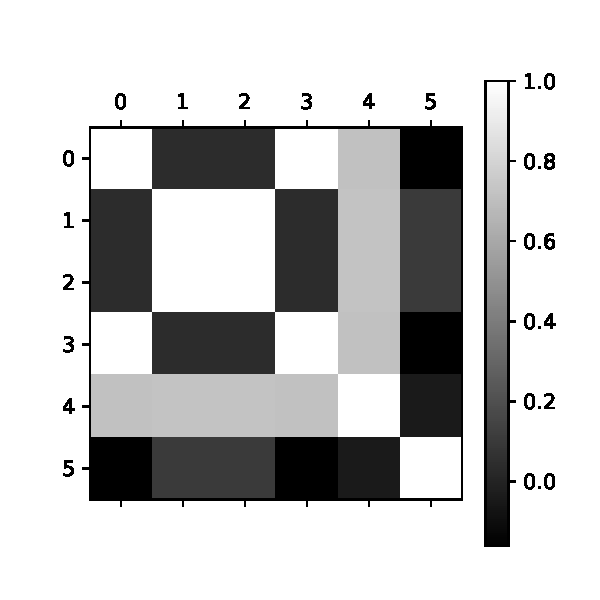
\includegraphics[width=0.5\textwidth]{plots/grabovoy/Cov.pdf}}
\subcaption{Матрица ковариации}
\end{minipage}
\begin{minipage}[t]{.5\textwidth}
{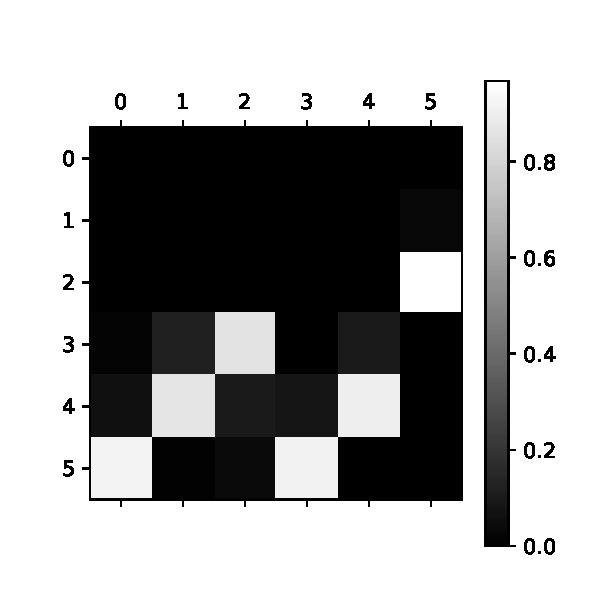
\includegraphics[width=0.5\textwidth]{plots/grabovoy/BelslyImage.pdf}}
\subcaption{Дисперсионные доли}
\end{minipage}
\caption{Илюстрация метода Белсли}
\label{CovBel}
\end{figure}

\begin{table}[h]
\begin{center}
\caption{Илюстрация метода Белсли}
\begin{tabular}{|c|cccccc|}
\hline
$\eta$ & $q_1$& $q_2$& $q_3$& $q_4$& $q_5$& $q_6$\\
\hline
$1.0$ &  $2\cdot 10^{-17}$ &  $4\cdot 10^{-17}$ &  $1\cdot 10^{-16}$ &  $2\cdot 10^{-17}$ &  $6\cdot 10^{-17}$&  $3\cdot 10^{-4}$ \\
\hline
$1.5$ &  $5\cdot 10^{-17}$ &  $9\cdot 10^{-17}$ &  $2\cdot 10^{-16}$ &  $5\cdot 10^{-17}$ &  $3\cdot 10^{-20}$ &  $3\cdot 10^{-2}$ \\
\hline
$3.3$ &  $9\cdot 10^{-18}$ &  $1\cdot 10^{-17}$ &  $2\cdot 10^{-17}$ &  $9\cdot 10^{-18}$ &  $2\cdot 10^{-19}$ &  $9\cdot 10^{-1}$ \\
\hline
$2\cdot 10^{15}$ &  $1\cdot 10^{-2}$ &  $1\cdot 10^{-1}$ &  $8\cdot 10^{-1}$ &  $2\cdot 10^{-3}$ &  $9\cdot 10^{-2}$ &  $1\cdot 10^{17}$ \\ 
\hline
$8\cdot 10^{15}$ &  $6\cdot 10^{-2}$ &  $8\cdot 10^{-1}$ &  $9\cdot 10^{-2}$ &  $8\cdot 10^{-2}$ &  $9\cdot 10^{-1}$ & $ 2\cdot 10^{17} $\\
\hline
$1\cdot 10^{16}$ &  $\bf9\cdot 10^{-1}$ &  $1\cdot 10^{-2}$& $ 4\cdot 10^{-2}$&  $\bf9\cdot 10^{-1}$ &  $1\cdot 10^{-3}$ & $ 5\cdot 10^{-21}$ \\
\hline
\end{tabular}
\label{CovBelTable}
\end{center}
\end{table}

Дисперсионный долевой коэффициент $q_{ij}$ определим как вклад $j$-го признака в дисперсию $i$-го элемента вектора параметра~$\textbf{w}$:

$$q_{ij} = \frac{u^2_{ij}/\lambda_{jj}}{\sum^n_{j=1}{u^2_{ij}/\lambda_{jj}}}. \eqno(4.3)$$

Большие значение дисперсионных долей указывают на наличие зависимости между параметрами. Находим долевые коэффициенты, которые вносят максимальный вклад в дисперсию параметра~$w_\xi$:

$$\zeta = \argmax_{j\in \mathcal{A}}{q_{\xi j}}. \eqno(4.4)$$
Параметр с индексом $\zeta$ определим как наименее релевантный параметр нейросети. 
%Для удаления нескольких зависимых параметров за раз, предлагается удалить параметры с номерами $p \in \mathcal{A}: q_{\xi i} > \lambda  \in  \mathbb{R}_+$.

Проиллюстрируем принцип работы метода Белсли на примере. Рассмотрим данные порожденные следующим образом: 
$$\textbf{w} = \begin{bmatrix}
\text{sin}(x)\\
\text{cos}(x)\\
\text{2+cos}(x)\\
\text{2+sin}(x)\\
\text{cos}(x) + \text{sin}(x)\\
x
\end{bmatrix}$$
с матрицей ковариации на рис.~\ref{CovBel}.a, где $x \in [0.0, 0.02, ..., 20.0]$.


В табл.~\ref{CovBelTable} приведены индексы обусловленности и соответствующие им дисперсионные доли, которые также изображены на рис.~\ref{CovBel}.b. Согласно этим данным, максимальный индекс обусловленности $\eta_6 = 1.2\cdot 10^{16}$. Ему соответствуют максимальные дисперсионные доли признаков с индексами 1 и 4, которые, как видно из построения выборки, коррелируют между собой.


\textbf{Вычислительный эксперимент. }
Для анализа свойств предложенного алгоритма и сравнения его с существующими был проведен вычислительный эксперимент в котором параметры нейросети удалялись методами,  которые были описаны в разделах 3.1---3.3 и методом Белсли.

В качестве данных использовались три выборки. Выборки Wine~\cite{Wine} и Boston~Housing~\cite{Boston}  --- это реальные данные. Синтетические данные сгенерированы таким образом, чтобы параметры сети были мультикоррелируемые. Генерация данных состояла из двух этапов. 
На первом этапе генерировался вектор параметров $\mathbf{w}_{\text{synthetic}}$:
$$\mathbf{w}_{\text{synthetic}}  \sim \mathcal{N}(\textbf{m}_{\text{synthetic}}, \textbf{A}_{\text{synthetic}}), \eqno(5.1)$$ 
где 
$\textbf{m}_{\text{synthetic}} = \begin{bmatrix}
1.0\\
0.0025\\
\cdots\\
0.0025
\end{bmatrix}$,
$\textbf{A}_{\text{synthetic}} = \begin{bmatrix}
1.0& 10^{-3}& \cdots& 10^{-3}& 10^{-3}\\
10^{-3}& 1.0& \cdots& 0.95& 0.95\\
\cdots&\cdots&\cdots&\cdots&\cdots\\
10^{-3}& 0.95& \cdots& 0.95& 1.0
\end{bmatrix}$.

На втором этапе генерировалась выборка $\mathfrak{D}_{\text{synthetic}}$:
$$\mathfrak{D}_{\text{synthetic}} = \{(\textbf{x}_i,y_i)| \textbf{x}_i \sim  \mathcal{N}(\textbf{1}, \textbf{I}), y_i = x_{i0}, i = 1 \cdots 10000\}. \eqno(5.2)$$
В приведенном выше векторе параметров $\mathbf{w}_{\text{synthetic}}$ для выборки $\mathfrak{D}_{\text{synthetic}}$, наиболее релевантным является первый параметр, а все остальные параметры являются нерелевантными. Матрица ковариации была выбрана таким образом, чтобы все нерелевантные параметры были зависимы и метод Белсли был максимально эффективен.



\begin{table}[h]

\begin{center}
\caption{Описание выборок}
\begin{tabular}{|c|c|c|c|}
\hline
	Выборка &Тип задачи& Размер выборки& Число признаков\\
	\hline
	
	\multicolumn{1}{|l|}{Wine}
	&
	\multicolumn{1}{|l|}{класификация}
	 & 178 & 13\\
	\hline
	
	\multicolumn{1}{|l|}{Boston Housing}
	&
	\multicolumn{1}{|l|}{регресия}
	& 506 & 13\\
	\hline
	
	\multicolumn{1}{|l|}{Synthetic data}
	&
	\multicolumn{1}{|l|}{регресия}
	& 10000 & 100\\
\hline

\end{tabular}
\end{center}
\end{table}



Для алгоритмов тренировочная и тестовая выборки составили~$80\%$ и~$20\%$ соответсвенно. Критерием качества прореживания служит процент параметров нейросети, удаление которого не влечет значимой потери качества прогноза. Также критерием качества служит устойчивость нейросети к зашумленности данных. 

Качеством прогноза $R_{\text{cl}}$ модели для задачи классификации является точность прогноза модели:
$$R_{\text{cl}} = \frac{\sum_{(\textbf{x},y)\in \mathfrak{D}} [f(\textbf{x}, \textbf{w}) = y]}{\left|\mathfrak{D}\right|}, \eqno(5.3)$$

Качеством прогноза $R_{\text{rg}} $ модели для задачи регрессии является среднеквадратическое отклонение результата модели от точного:

$$R_{\text{rg}} = \frac{\sum_{(\textbf{x},y)\in \mathfrak{D}} \left(f(\textbf{x}, \textbf{w}) - y\right)^2}{\left|\mathfrak{D}\right|}, \eqno(5.4)$$

\textbf{Wine.} Рассмотрим нейроную сеть с 13 нейронами на входе, 13 нейронами в скрытом слое и 3 нейронами на выходе.

\begin{figure}[h!t]\center
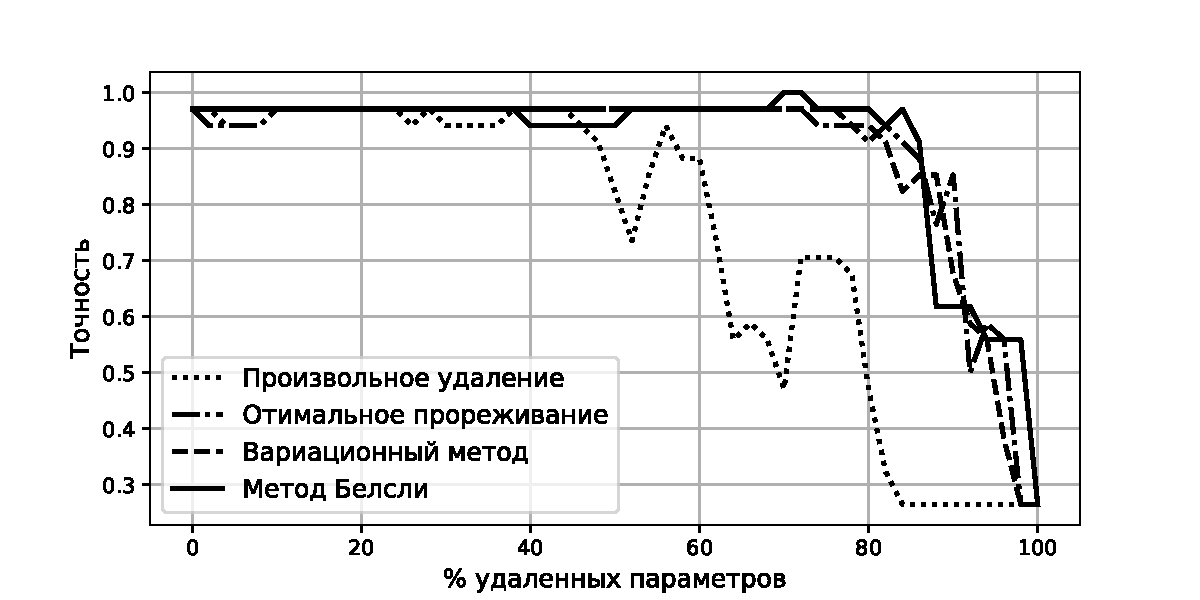
\includegraphics[width=0.8\textwidth]{plots/grabovoy/Wine/All.pdf}\\
\caption{Качество прогноза при удаление параметров на выборке Wine}
\label{WineAll}
\end{figure}

\begin{figure}[h!t]\center
\begin{minipage}[t]{.5\textwidth}
{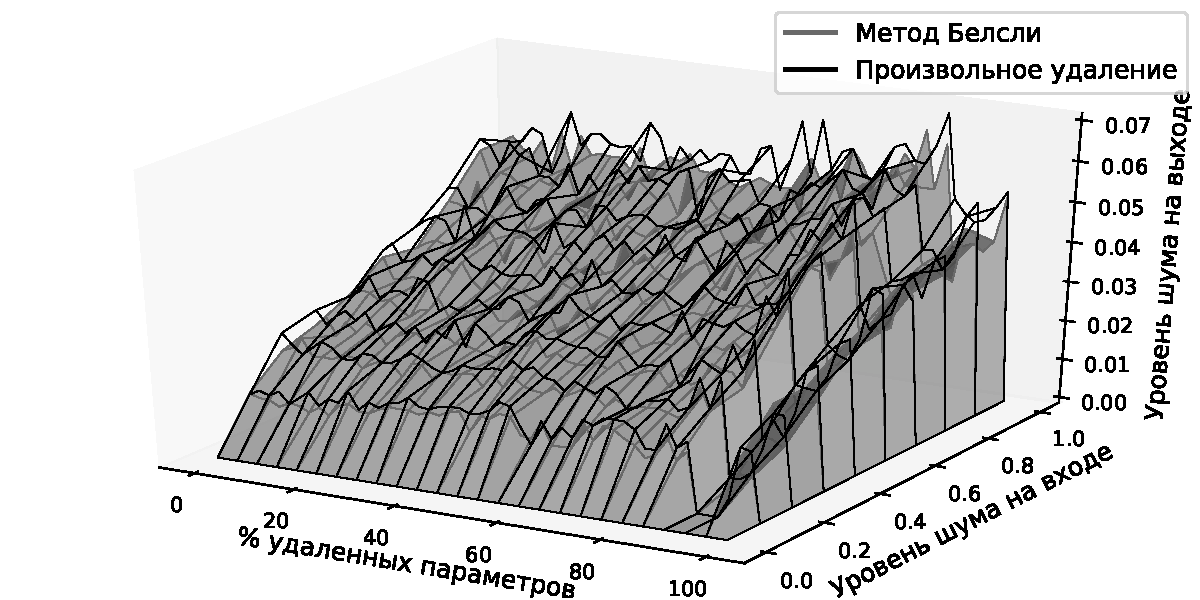
\includegraphics[width=0.5\textwidth]{plots/grabovoy/Wine/RandomNoise3D.pdf}}
\subcaption{Произвольное удаление параметров}
\end{minipage}

\begin{minipage}[t]{.5\textwidth}
{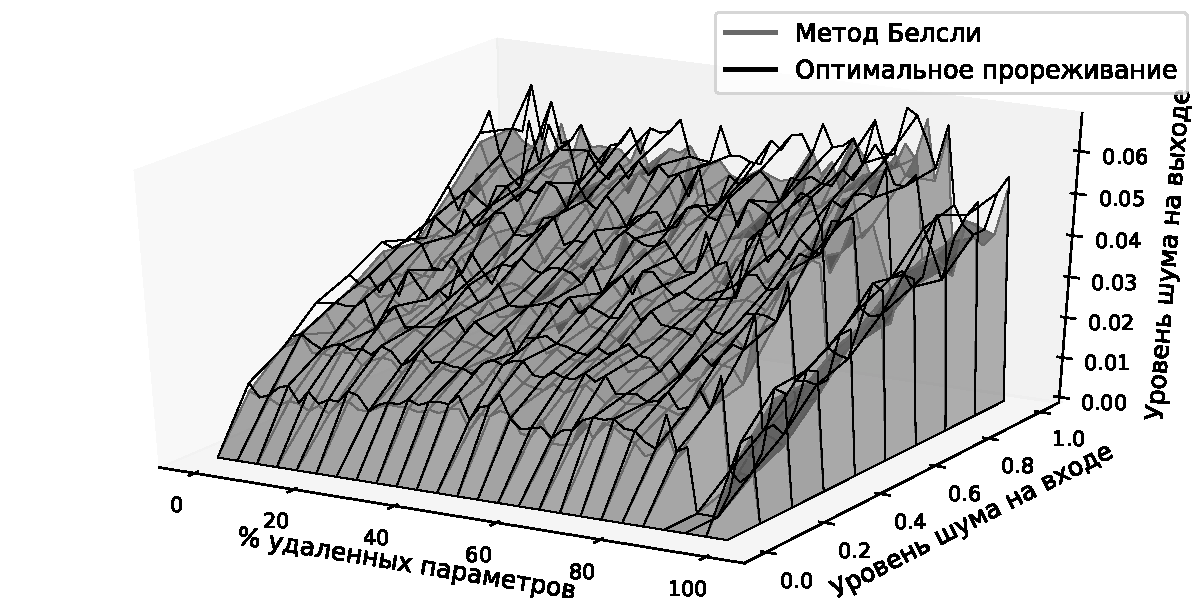
\includegraphics[width=0.5\textwidth]{plots/grabovoy/Wine/OBDNoise3D.pdf}}
\subcaption{Оптимальное прореживание}
\end{minipage}

\begin{minipage}[t]{.5\textwidth}
{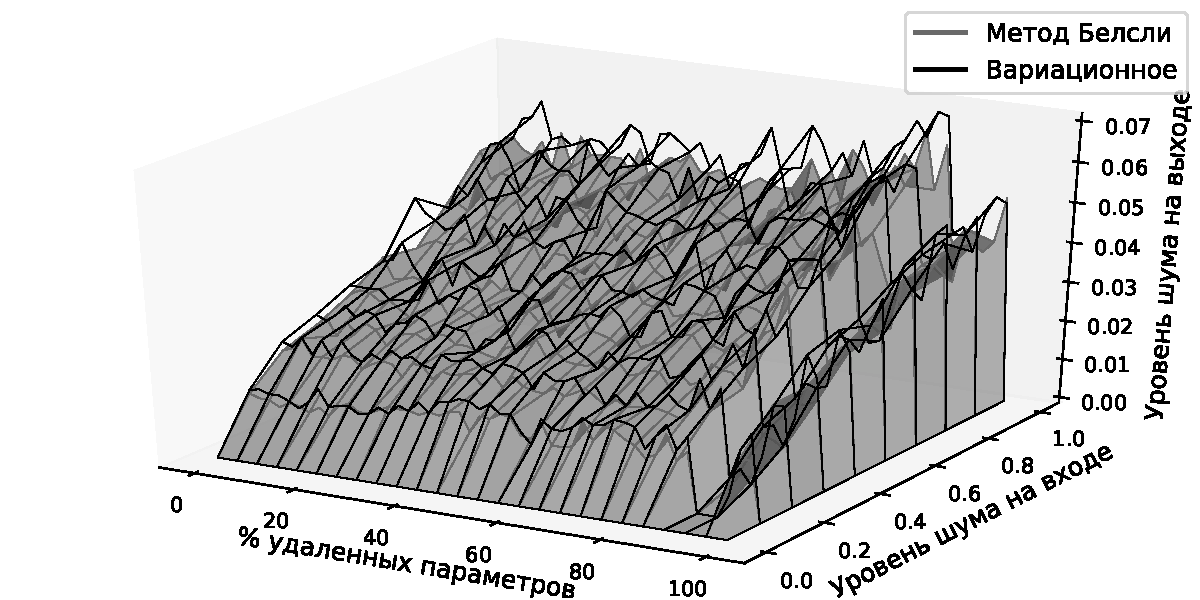
\includegraphics[width=0.5\textwidth]{plots/grabovoy/Wine/VariationalNoise3D.pdf}}
\subcaption{Вариационный метод}
\end{minipage}

\label{WineNoise}
\caption{Влияние шума в начальных данных на шум выхода нейросети на выборке Wine}
\end{figure}

На рис.~\ref{WineAll} показано как меняется точность прогноза $R_{\text{cl}}$ при удалении параметров указанными методами. Из графика видно, что метод оптимального прореживания, вариационный метод и метод Белсли позволяют удалить $\approx80\%$ параметров и качество всех этих методов падает при удалении $\approx90\%$ параметров нейросети. 

На рис.~\ref{WineNoise} показаны поверхности изменения уровня шума ответов нейросети при изменении процента удаленных параметров и уровня шума входных данных для разных методов прореживания. На графиках показано, что при удалении параметров нейросети методом Белсли шум меньше, чем при удалении параметров другими методами, на это указывает то что поверхность которая соответствует методу Белсли ниже других поверхностей.

\textbf{Boston Housing.} Рассмотрим нейроную сеть с 13 нейронами на входе, 39 нейронами в скрытом слое и одним нейроном на выходе.

\begin{figure}[h!t]\center
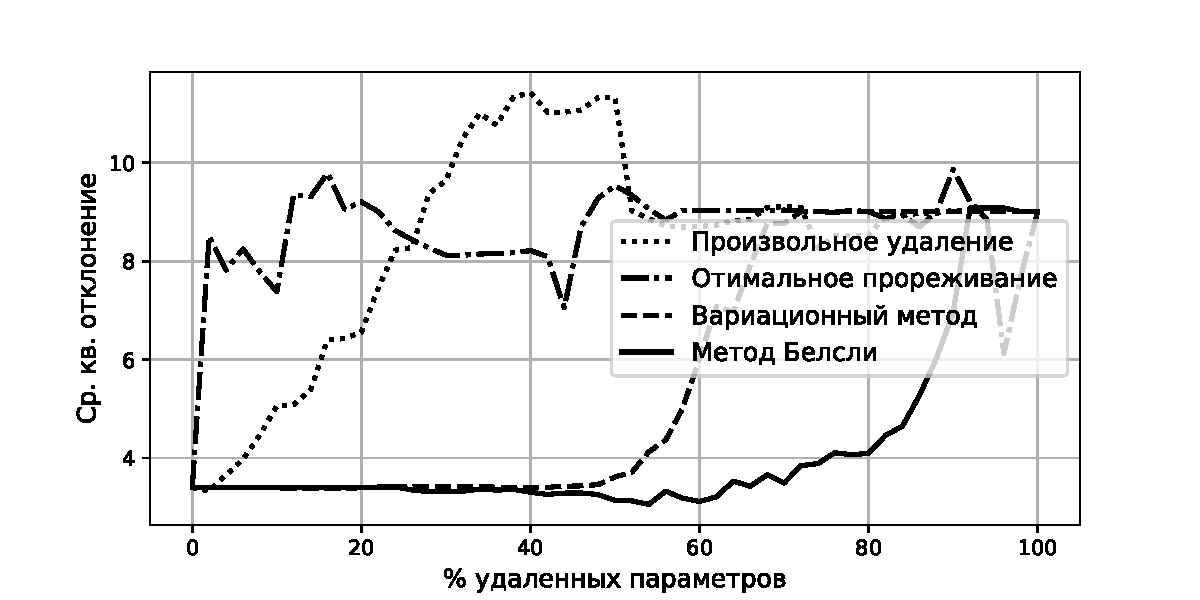
\includegraphics[width=0.8\textwidth]{plots/grabovoy/Boston/All.pdf}\\
\caption{Качество прогноза при удаление параметров на выборке Boston}
\label{BostonAll}
\end{figure}


\begin{figure}[h!t]\center
\begin{minipage}[t]{.5\textwidth}
{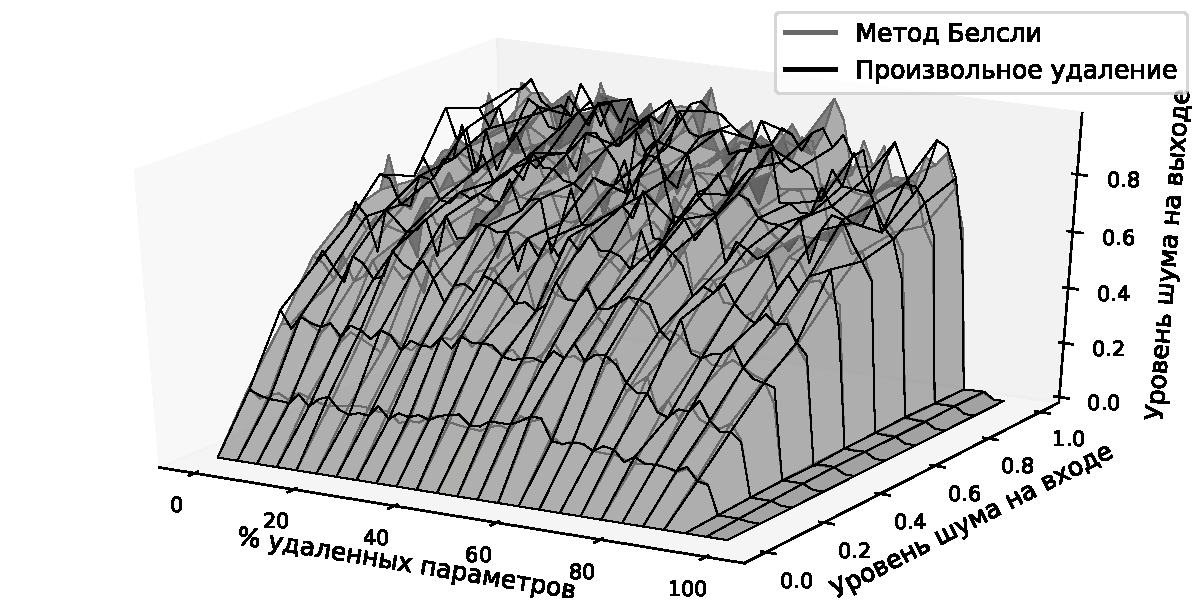
\includegraphics[width=0.5\textwidth]{plots/grabovoy/Boston/RandomNoise3D.pdf}}
\subcaption{Произвольное удаление параметров}
\end{minipage}
\begin{minipage}[t]{.5\textwidth}
{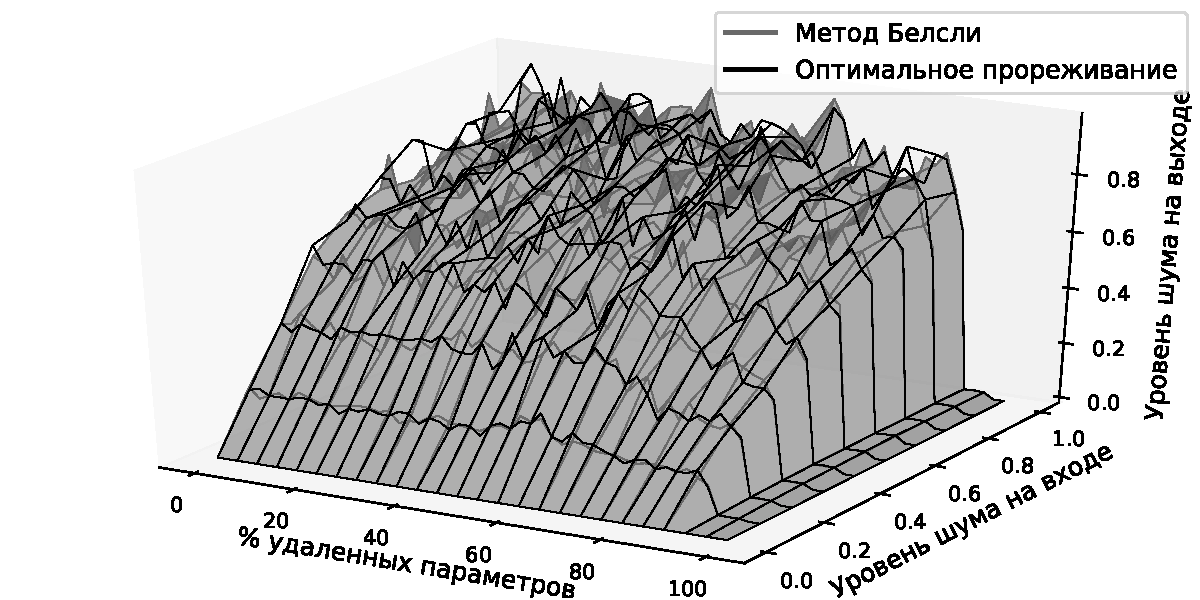
\includegraphics[width=0.5\textwidth]{plots/grabovoy/Boston/OBDNoise3D.pdf}}
\subcaption{Оптимальное прореживание}
\end{minipage}

\begin{minipage}[t]{.5\textwidth}
{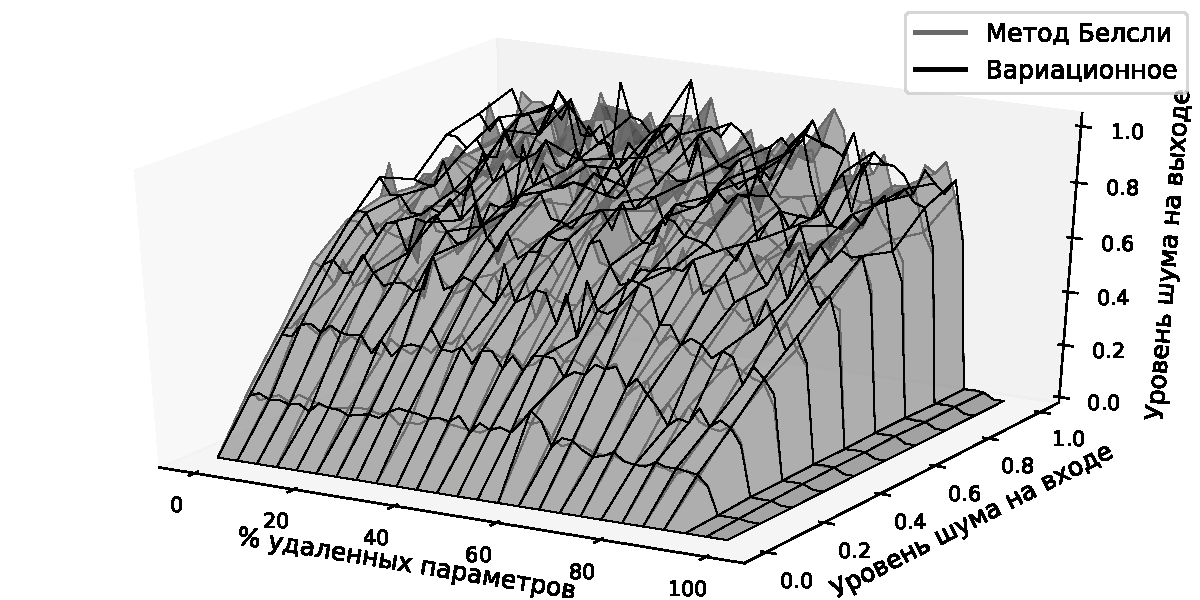
\includegraphics[width=0.5\textwidth]{plots/grabovoy/Boston/VariationalNoise3D.pdf}}
\subcaption{Вариационный метод}
\end{minipage}

\caption{Влияние шума в начальных данных на шум выхода нейросети на выборке Boston}
\label{BostonNoise}
\end{figure}


На рис.~\ref{BostonAll} показано как меняется среднеквадратическое отклонение прогноза $R_{\text{rg}}$ от точного ответа  при удалении параметров указанными методами. График показывает, что метод Белсли является более эффективным, чем другие методы, так-как позволяет удалить больше параметров нейросети без потери качества.

На рис.~\ref{BostonNoise} показаны поверхности изменения уровня шума ответов нейросети при изменении процента удаленных параметров и уровня шума входных данных для разных методов прореживания. График показывает, что уровень шума всех методов одинаковый, так как поверхности всех методов находятся на одном уровне.


\textbf{Синтетические данные.} Рассмотрим нейроную сеть с 100 нейронами на входе и одним нейроном на выходе.

\begin{figure}[h!t]\center
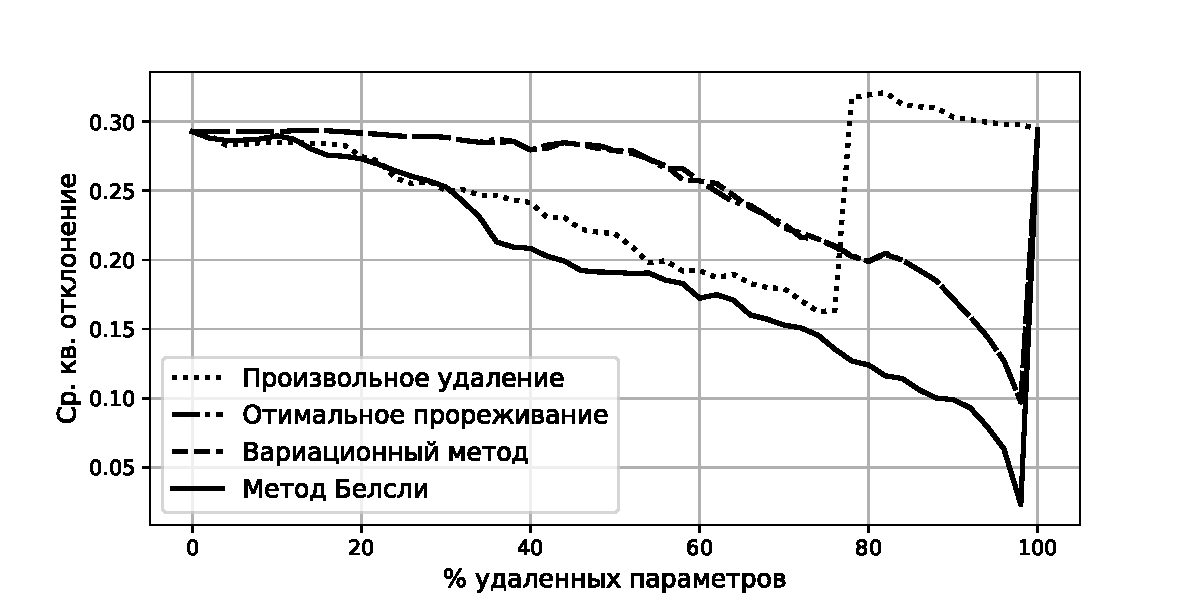
\includegraphics[width=0.8\textwidth]{plots/grabovoy/Data1/All.pdf}\\
\caption{Качество прогноза при удаление параметров на синтетической выборке}
\label{Data1All}
\end{figure}

\begin{figure}[h!t]\center
\begin{minipage}[t]{.5\textwidth}
{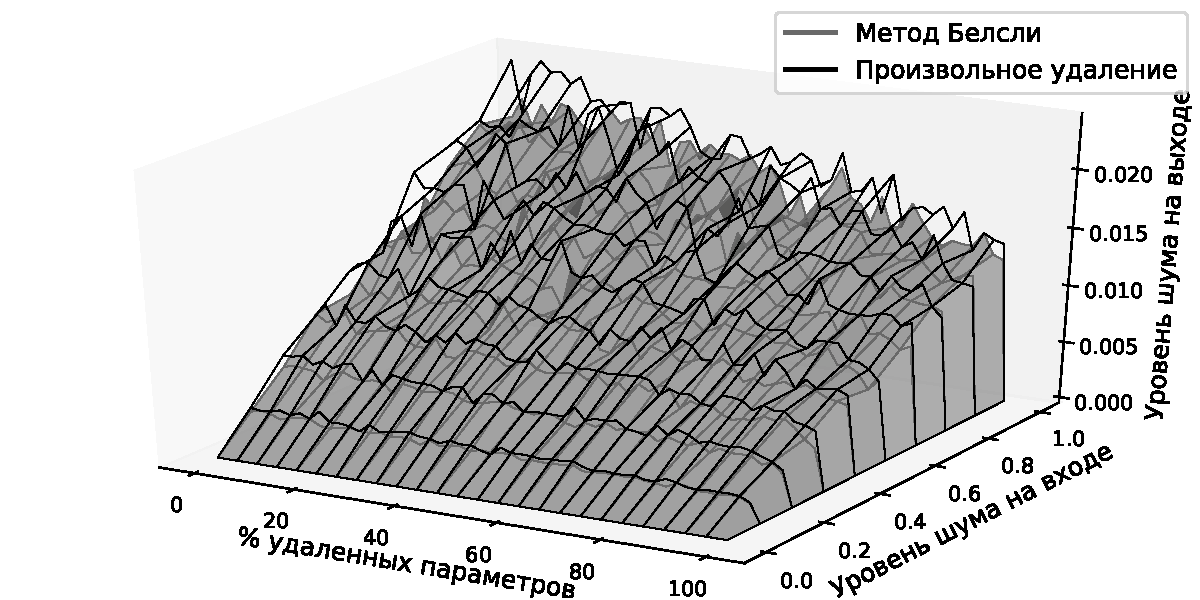
\includegraphics[width=0.5\textwidth]{plots/grabovoy/Data1/RandomNoise3D.pdf}}
\subcaption{Произвольное удаление параметров}
\end{minipage}
\begin{minipage}[t]{.5\textwidth}
{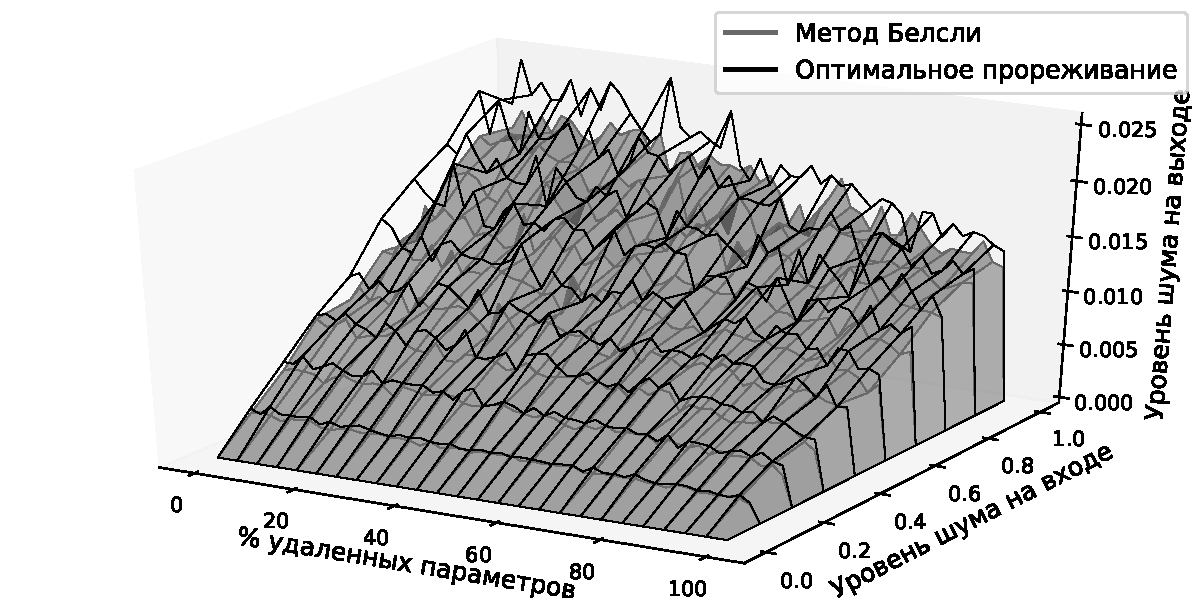
\includegraphics[width=0.5\textwidth]{plots/grabovoy/Data1/OBDNoise3D.pdf}}
\subcaption{Оптимальное прореживание}
\end{minipage}

\begin{minipage}[t]{.5\textwidth}
{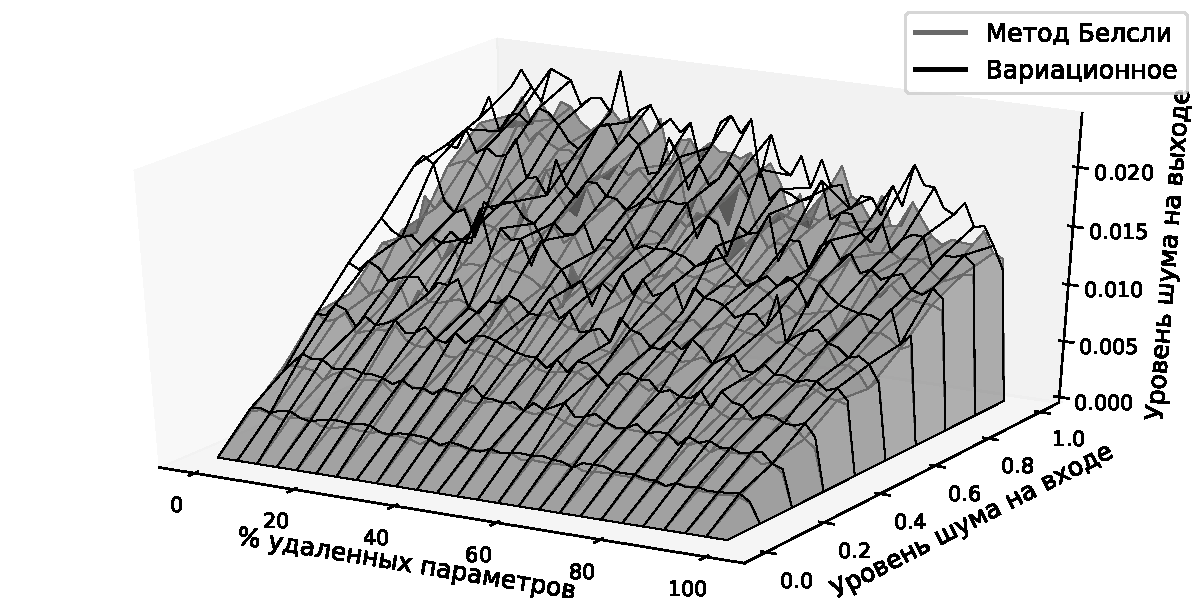
\includegraphics[width=0.5\textwidth]{plots/grabovoy/Data1/VariationalNoise3D.pdf}}
\subcaption{Вариационный метод}
\end{minipage}

\caption{Влияние шума в начальных данных на шум выхода нейросети на синтетической выборке}
\label{Data1Noise}
\end{figure}


На рис.~\ref{Data1All} показано как меняется среднеквадратическое отклонение прогноза от $R_{\text{rg}}$ точного ответа при удалении параметров указанными методами. График показывает, что удаление параметров методом Белсли являеться более эффективным чем другие методы прореживания, так-как качество прогноза нейросети улучшается при удалении шумовых параметров.

На рис.~\ref{Data1Noise} показаны поверхности изменения уровня шума ответов нейросети при изменении процента удаленных параметров и уровня шума входных данных для разных методов прореживания. На графиках показано, что при удалении параметров нейросети методом Белсли шум меньше, чем при удалении параметров другими методами, так-как поверхность которая соответствует методу Белсли ниже других поверхностей.

